\documentclass[
12pt,
a4paper,
twoside
% fullpage 
]{report}

\usepackage{xcolor}

% \definecolor{ediblue}{RGB}{22,39,74} 
\definecolor{ediblue}{RGB}{0,79, 113} 
% \definecolor{edired}{RGB}{172,0,64} 
\definecolor{edired}{RGB}{214,30,56} 
\definecolor{edipurple}{RGB}{208,0,111} 


\definecolor{figcaption}{RGB}{58, 59, 60} 





\usepackage{graphics}
\usepackage{epsf,graphicx}%, amstext,url} 
\usepackage{pdfpages}
\usepackage{amsmath}
\usepackage{float}
% \usepackage{todonotes}
\usepackage[colorinlistoftodos]{todonotes}
\usepackage{listings}
\usepackage{cancel}
\usepackage{url}
\usepackage[version=4]{mhchem}
\bibliographystyle{unsrt}
\usepackage{lipsum}
\setlipsum{%
  % par-before = \begingroup\color{lightgray},
  % par-after = \endgroup
}


% DO NOT SWITCH ORDER OF THESE PACKAGES 
\usepackage{tikz}
\usepackage{amsmath} % for \dfrac
\usepackage{bm} % \bm
\usepackage{physics}
\usepackage{tikz,pgfplots}
\usepackage[outline]{contour} % glow around text
\usetikzlibrary{angles,quotes} % for pic (angle labels)
\usetikzlibrary{calc}
\usetikzlibrary{decorations.markings}
\usetikzlibrary{patterns,snakes}
\tikzset{>=latex} % for LaTeX arrow head
\contourlength{1.6pt}
\colorlet{Bcol}{violet!90}
\colorlet{BFcol}{red!60!black}
\colorlet{Scol}{green!60!black}
\colorlet{veccol}{green!45!black}
\colorlet{Icol}{blue!70!black}
\colorlet{mucol}{red!90!black}
\tikzstyle{BField}=[->,thick,Bcol]
\tikzstyle{current}=[->,Icol] %thick,
\tikzstyle{force}=[->,thick,BFcol]
\tikzstyle{vector}=[->,thick,veccol]
\tikzstyle{mu vector}=[->,thick,mucol]
\tikzstyle{spin}=[->,very thick,Scol]
\tikzstyle{velocity}=[->,very thick,vcol]
\tikzstyle{charge+}=[very thin,draw=black,top color=red!50,bottom color=red!90!black,shading angle=20,circle,inner sep=0.5]
% \tikzstyle{charge-}=[very thin,draw=black,top color=blue!50,bottom color=blue!80,shading angle=20,circle,inner sep=0.5]
\tikzstyle{metal}=[top color=black!15,bottom color=black!25,middle color=black!5,shading angle=10]
\tikzset{
  BFieldLine/.style={thick,Bcol,decoration={markings,mark=at position #1 with {\arrow{latex}}},
                                 postaction={decorate}},
  BFieldLine/.default=0.5,
  pics/magnet/.style={ %args={#1}
    code={
      \def\h{0.9}
      \coordinate (-N) at (0,\h);
      \coordinate (-S) at (0,-\h);
      \draw[pic actions,thick,top color=red!60,bottom color=red!90,shading angle=20]
        (-0.8*\h/2,0) rectangle ++(0.8*\h,\h);
      \draw[pic actions,thick,top color=blue!60,bottom color=blue!90,shading angle=20]
        (-0.8*\h/2,0) rectangle ++(0.8*\h,-\h);
      \node[pic actions] at (0, \h/2) {\textbf{N}};
      \node[pic actions] at (0,-\h/2) {\textbf{S}};
  }},
}

\colorlet{Ecol}{ediblue}
\colorlet{EcolFL}{ediblue}
\colorlet{Bcol}{blue!90!black}
\tikzstyle{EcolEP}=[blue!80!white]
\colorlet{veccol}{green!45!black}
\tikzstyle{charge+}=[very thin,top color=red!50,bottom color=red!90!black,shading angle=20]
\tikzstyle{charge-}=[very thin,top color=blue!50,bottom color=blue!80,shading angle=20]
\tikzstyle{charged}=[very thin,top color=purple!50,bottom color=purple!80,shading angle=20]
\tikzstyle{vector}=[->,thick,veccol]
\tikzset{EFieldLineArrow/.style={EcolFL,decoration={markings,mark=at position #1 with {\arrow{latex}}},
                                 postaction={decorate}},
         EFieldLineArrow/.default=0.5}
\def\R{1.8}
\def\NE{8}
\def\NV{4}
\contourlength{1.6pt}

\colorlet{veccol}{ediblue}
\colorlet{myblue}{blue!60!black}
\tikzstyle{vector}=[->,thick,veccol]
\def\R{1.4}
\def\r{0.03}
\def\N{9}

\usepackage{physics}
\usepackage{siunitx}

\colorlet{wavecol}{orange!35!black}
\colorlet{freqcol}{green!25!black}
\colorlet{enercol}{blue!35!black}
\pgfdeclareverticalshading{rainbow}{100bp}{
  color(0bp)=(red); color(25bp)=(red); color(35bp)=(yellow);
  color(45bp)=(green); color(55bp)=(cyan); color(65bp)=(blue);
  color(75bp)=(violet); color(100bp)=(violet)
}


\usepackage{braket}
%%%%%%%%%%%%%%%%%%%%%%%%%%%%%%%%%%%%%%%%%%%



% \usepackage[top=2cm,bottom=4cm,left=1.5cm,right=3cm,asymmetric]{geometry}
\usepackage[a4paper,width=165mm,top=25mm,bottom=25mm]{geometry}
\newcommand{\td}[1]{\todo[]{#1}}
\newcommand{\tdr}[1]{\todo[color=red]{#1}}
\newcommand{\tdg}[1]{\todo[color=green]{#1}}

\usepackage{fancyhdr}

\usepackage{setspace}
% \doublespacing
\onehalfspacing

\usepackage{imakeidx}
% \makeindex
\makeindex[columns=2, title=Index, intoc]
% \usepackage{hyperref}

\RequirePackage[hidelinks]{hyperref} % 

\hypersetup{
    colorlinks=true,
    % linkcolor=ediblue, 
    % citecolor=edipurple,
    linkcolor=edired, 
    citecolor=ediblue,
}

\usepackage{letltxmacro}
\LetLtxMacro{\originaleqref}{\eqref}
\def\eqref#1{%
\begingroup\hypersetup{
    linkcolor=edipurple,
    linkbordercolor=edipurple,
    }\originaleqref{#1}\endgroup
}

\usepackage{sectsty}
\usepackage[LGR, T1]{fontenc}
\usepackage{CrimsonPro}
\usepackage[default]{sourcesanspro}
\allsectionsfont{\rmfamily}


\usepackage{wrapfig}
\usepackage[font={color=figcaption,md},figurename=Fig.,labelfont={it}]{caption}


\begin{document}


\thispagestyle{empty}

%
%	This is a basic LaTeX Template for the TP/MP MSc Dissertation report

\parindent=0pt          %  Switch off indent of paragraphs 
\parskip=5pt            %  Put 5pt between each paragraph  

% \documentclass[
12pt,
a4paper,
% fullpage 
]{report}
\usepackage{graphics}
\usepackage{epsf,graphicx}%, amstext,url} 
\usepackage{afterpage}
\begin{document}
%	This section generates a title page
%       Edit only the sections indicated to put in the project title, and submission date
\begin{titlepage}
\vspace*{0.1\textheight}

\begin{center}
        \huge{\bfseries Title of my Dissertation}\\ % Replace with the title of your dissertation!
\end{center}

\medskip

\begin{center}
        \Large{Conner J Adlington}\\  % Author of dissertation - replace with your name!
        \medskip
        \large{August XX, 2024}  % Submission date
\end{center}

%%% If necessary, reduce the number 0.4 below so the University Crest
%%% and the words below it fit on the page.
%%% Don't let the crest, or the wording below it, flow onto the next page!

\vspace*{0.3\textheight}

\begin{center}
        \includegraphics[width=35mm]{../crest.pdf}
\end{center}

\medskip

\begin{center}

%%%
%%% Change Theoretical to Mathematical if appropriate
%%%
\large{
  MSc in Theoretical Physics\\[0.8ex]
  The University of Edinburgh\\[0.8ex]
  2023}

\end{center}

\end{titlepage}

\end{document}

\includepdf[pages=-]{Title/title.pdf}

\pagenumbering{roman}

This is where you summarise the contents of your dissertation. It should be
at least 100 words, but not more than 250 words.




\begin{center}
\textbf{Declaration}
\end{center}

I declare that this dissertation was composed entirely by myself.

% Chapters 2 and 3 provide an introduction to the subject area and a
% description of previous work on this topic. They do not contain
% original research.
%
% Chapter~4 describes work that was carried out entirely by me. The results of
% this chapter have been obtained previously by Professor Anne T Matta of the
% University of Kinlochteuchter, but the methods used here are different
% in some important (or minor) ways.
%
% Chapters 4 through 6 contain my original work. The work described in
% Chapter~4 was carried out in collaboration with Professor Carole Ann O'Malley
% and her PhD student Jack O'Bean. Chapter~5 presents original work done
% entirely by me.
%
% \bigskip
%
% State whether calculations were done using Mathematica, Maple, MATLAB,
% SymPy, etc, with (or without) gamma-matrix manipulation code, master
% integrals, the Super-Duper software package, etc. In other words, you
% should refer to any software that you used during your project. For
% example, Monte Carlo simulation packages, hydrodynamics packages,
% measurement code, fitting code, tensor algebra and/or calculus packages,
% Feynman diagram evaluation packages, etc.
%
% State whether any software you used was written by you from scratch,
% by your supervisor (or by whoever), or if it's a standard package.
%
\newpage
%
%


\topskip0pt
\vspace*{\fill}
\begin{center}
\textrm{\bfseries\Huge Personal Statement}%
\end{center}%

\vspace{1em}

% \emph{You \textbf{\emph{must}} include a Personal Statement in your
%   dissertation. This should describe what you did during the project,
%   and when you did it. Give an account of problems you faced and how
%   you attempted to overcome them. The examples below are based on
%   personal statements from MSc and MPhys projects in previous years,
%   with (mostly-obvious) changes to make them anonymous. }
%
The project began with developing a deeper understanding of the physics underlying spintronics. 
The focus was on electron paramagnetic resonance (EPR), specifically using the continuous wave optically detected magnetic resonance technique (CW-ODMR). For this, there is a wealth of literature on the diamond nitrogen vacancy (DNV). Most popular is the application of the DNV as a very sensitive magnetometer. 

I worked to  understand the intricacies of the diamond systems, with the intention of applying this knowledge to SiC. 
When I felt comfortable with the underlying physics, I began modelling the different system Hamiltonians. I applied varying $\vec{B}$ and $\vec{E}$ as well as varied temperature. The goal was both to understand the influence of these external factors on the spin-system energy levels as well as to verify my model behaved correctly in the simple cases when compared to existing literature. 

When I had the capability to dynamically model both the DNV and several SiC defects, with different spin numbers, I created ensembles of specifically chosen defects to visualise how the CW-ODMR spectra might change under the influence of varying $\vec{B}$, $\vec{E}$ and $T$. This, as well as existing literature allowed me to isolate specific defects which were most appropriate for the sensing of specific variables. 
For example, the V2 Silicon defect in SiC is very insensitive to changes in temperature so would not be the most appropriate for thermometry application. 

When an ensemble of defects was selected for a specific multi-modal application and the nature of the changes to the ODMR spectra was understood, I worked to develop a method to extract and disentangle the influence of each individual influence on the spectra. 

This process was repeated for several model systems and in the end I developed multimodal sensing techniques for specifically chosen defects and external parameters in SiC. In some cases the freedom of the parameters was scoped (i.e. fixing a field direction), however as discussed in the analysis, this still provides value. 

During the course of the project, I met with my supervisor every week,
in order to discuss my progress and the direction I would head
next. Toward the end, the frequency of our meetings increased
somewhat, as I began to finish my investigations.

I started writing this dissertation in early-July, determined to give a solid overview of the field, then I spent the all of August working on it full-time.

Overall, I feel that the project was a success, and I found it to be
extremely enjoyable throughout.


% \subsubsection*{Example~1: an analytical project}
%
% The project began with an introduction to the spinor-helicity
% formalism in four dimensions, with my main source material being
% H. Elvang's “Scattering Amplitudes in Gauge Theory and Gravity” [1]. I
% read the first chapter, and acquainted myself with the formalism,
% and how it worked in a practical sense.
%
% Once I felt more comfortable with it, we moved onto the
% six-dimensional spinor-helicity formalism paper, where I spent some
% time gaining as strong an understanding of how the formalism worked,
% and proving identities.
%
% The next stage was to learn about the generalised unitarity procedure,
% with the end goal being to use it to calculate coefficients for some
% one loop integral, likely involving massive particles. Learning how
% this worked took some time, and proved to be some of the most
% difficult material for me to understand.
%
% It wasn't until later that we began to consider applying what I had
% learned to a Kaluza-Klein reduction, which ended up being the main
% focus of the project. It mixed well with the general theme of
% “extra-dimensional theory” the project began with, and allowed me to
% apply all that I'd learned and prepared for so far.  The vast majority
% of my remaining time was spent calculating coefficients for the scalar
% box contribution to the gluon-gluon to two-Kaluza-Klein-particle
% amplitude, overcoming a number of problems and errors, to finally have
% human-readable, and presentable results.
%
% During the course of the project, I met with my supervisor every week,
% in order to discuss my progress and the direction I would head
% next. Toward the end, the frequency of our meetings increased
% somewhat, as I began to finish my calculations.
%
% I started writing this dissertation in mid-July, and I spent the first
% three weeks of August working on it full-time.
%
% Overall, I feel that the project was a success, and I found it to be
% extremely enjoyable throughout.
%
%
% \subsubsection*{Example~2: a computational project}
%
% I spent the first 2 weeks of the project reading the material
% surrounding my project - mainly [1] and [2]. I also began to plan out
% how I would implement the algorithms in C++, in doing this I gained an
% understanding of what the main goals of the first half of my project
% would be and how they could be achieved. I identified which Monte
% Carlo observables would be useful to measure in these simulations.
%
% For the next 3 weeks I implemented the standard Atlantic City
% algorithm and debugged my code whilst developing analysis tools in
% python. I compared the results from my simulations to the results from
% [3] (for the Random Osculator) and [4] for the EvenMoreRandom
% Osculator. Having obtained positive results for the Random Osculator I
% started reading up on Heaviside Articulation. I examined how to
% integrate a Heaviside Articulator into the simulation in order to
% produce the most efficient simulation - the solution I decided on was
% to use a package called HeaviArt[5].
%
% Following this I began to integrate the Heaviside Articulator into my
% code and test it against the regular algorithm. In addition to this I
% ran longer simulations to verify my findings without Articulation.
%
% In mid July I finished implementing Heaviside Articulation into my
% code and began looking into how to quantify any improvement in speed
% gained by this algorithm. As July progressed I started looking into
% how to integrate the EvenMoreRandom Osculator into my code - this was
% the most complicated part of the project, as discussed in the body of
% this report. Despite much effort on my part, I couldn't get the
% results produced by the new algorithm to agree with the old
% ones. Following further study of the literature, and long discussions
% with Jack O'Bean, it turned out that the original form of Heaviside
% Articulation didn't applied to the EvenMoreRandom Osculator. With the
% help of Jack and my supervisor, I then developed the new version
% described in this report. I also did analytical calculations of the
% four-point blue function to two orders higher than had
% been published previously in the literature.
%
% For the final parts of the summer I worked mainly on perfecting the
% algorithm for the Random Osculator and implementing the EvenMoreRandom
% Osculators algorithm with the improved Heaviside Articulation. The
% final results were encouraging, but more work is clearly needed. To
% this end, I have been awarded a studentship by the British University
% of Lifelong Learning to extend this work during my PhD Studies at
% the non-existent Scottish Highlands Institute of Technology in
% Inveroxter.
%
% I started writing this dissertation in mid-July, and I spent the first
% three weeks of August working on it full-time.
%
%
% \subsubsection{Example~3: a more mathematical project}
%
% My first two weeks of work on the project consisted of building up a
% working knowledge of the algebraic structures and techniques which
% would be used in the main calculations which were to be carried out,
% in particular carefully reading up on the 11-dimensional case [1, 2],
% the general structure of the Spencer complex of the Poincar\'e
% superalgebra, the Clifford and exterior algebras over a Lorentzian
% vector space in general finite dimension and the relationship between
% them, the spin group, the Lorentz algebra $so(V$) and their vector and
% spinor representations. As a toy calculation, I computed the first two
% Spencer cohomology groups of the Poincar\'e algebra and its relevant
% subalgebras in order to find its filtered (sub)deformations, finding
% that these are given by a space of algebraic curvature operators. This
% calculation is vastly simplified compared to the superalgebra
% calculation owing to the lack of spinor structure.
%
% In the following two weeks, I turned to the particular case of 5
% dimensions, initially study- ing the quaternionic structure of the
% relevant Clifford algebra, its spinor representation and symplectic
% Majorana spinors. I read up on complex and quaternionic structures and
% representations, proved various identities for products of higher-rank
% gamma matrices found in [5] and derived the Fierz identity and various
% other useful identities involving quantities defined in terms of the
% Majorana spinors. I made an initial attempt to solve the relevant
% cocycle conditions, initially finding that the space of solutions was
% given by 3-forms (or Hodge-dually 2-forms), but from the known spinor
% connection in D = 5 supergravity we knew that there was a problem with
% the solution. Working with my supervisor to fix the errors in this
% calculation, finding the most efficient way of setting it out and
% writing up the work done so far and some of the background material
% took up the following two to three weeks.  Next, I moved on to
% figuring out the fundamentals of the geometric part of the project,
% understanding spin structures on manifolds, the spin lift of the
% Levi-Civita connection, the spinorial Lie derivative and the
% definition of the superconnection. I derived the flatness conditions
% for the curvature of the superconnection and showed that these
% conditions are sufficient to cause the Killing superalgebra to close
% and form a Lie superalgebra. This work, along with further writeup,
% took another two weeks.
%
% The final weeks of the project were spent learning about Lorentzian
% and Riemannian symmetric spaces, finding all of the the maximally
% supersymmetric backgrounds, on the way learning a little about the
% supersymmetric solutions of 5-dimensional supergravity, and finally
% finishing the dissertation.
%

\todo[inline, color=red]{Review before submission}
\vspace*{\fill}
\newpage


\begin{center}
%\vspace*{2in}
% an acknowledgements section is completely optional but if you decide
% not to include it you should still include an empty {titlepage}
% environment as this initialises things like section and page numbering.
\textbf{Acknowledgements}
\end{center}
%
% \emph{Put your acknowledgements here. Thanking your supervisor for
% his/her help is standard practice, but it's not compulsory \ldots}
%
% I'd like to thank my supervisor Professor Carole Ann O'Malley for
% making this project possible, and her PhD student Jack O'Bean for his
% patience and his detailed functional explanations of how classical
% symmetries can be broken by quantum effects. Thanks also to Wally Bee
% and Ken Garoo of the University of Woolloomooloo for sending me
% their higher-order hopping-parameter expansions.
%
% Finally, none of this would have been possible without financial
% support from Paterson's Lane Education Committee.
%
% \bigskip
%
% This document has its origins in the dissertation template for the MSc
% in High Performance Computing, which is apparently descended from a
% template developed by Professor Charles Duncan for MSc students in
% Meteorology. His acknowledgement follows:
%
% \emph{This template has been produced with help from many former
%   students who have shown different ways of doing things. Please make
%   suggestions for further improvements.}
%
% Some parts of this template were lifted unashamedly from the Edinburgh
% MPhys project report guide, with little or no modification. I have no
% idea who wrote the first version of that\ldots
%
% You don't have to use \LaTeX\ for your dissertation. You can use
% Microsoft Word, Apple Pages, LibreOffice or similar, but it's
% \emph{much} easier to typeset equations in \LaTeX, and references look
% after themselves. Whatever you use, your dissertation should have the
% general structure of this template, and it should look similar --
% especially the front page.
%




\listoftodos
\tableofcontents
% \listoftables
\listoffigures
% \clearpage
\cleardoublepage

\pagestyle{fancy}
\fancyhf{}
\fancyhead[RE]{\rmfamily\nouppercase{\rightmark}}
\fancyhead[LO]{\rmfamily\nouppercase{\leftmark}}
\fancyhead[LE,RO]{\rmfamily\thepage}
\pagenumbering{arabic}

\chapter{Introduction}

% The Introduction should contain a description of your project and the
% problem you are trying to solve. It should start off at a level that
% should be understandable by anyone with a degree in physics, but it
% can become more technical later
%
% Where appropriate you should include references to work that has
% already been done on your topic and anything else which lets you set
% your work in context.
%
% One of the things you will need to do is to ensure that you have a
% suitable list of references.  To do this you should see \cite{Simon2013-lh}
% or some other suitable reference.  Note the format of the citation used
% here is the style favoured in this School.  Here is another
% reference \cite{Simon2013-lh} for good measure.
%
%
% You will also want to make sure you have no spelling or grammatical
% mistakes. To help identify speling mistukes you can use the commands
% \emph{aspell}, \emph{ispell} or \emph{spell} on most Linux/Unix
% computers. See the appropriate manual pages. Remember that spelling
% mistakes are not the only errors which can occur. Spelling checkers
% will not find errors which are, in fact, valid words such as
% \emph{there} for {\em their}, nor will they find repeated repeated
% words which sometimes occur if your concentration is broken when
% typing. \textbf{There is no substitute for thorough proof reading!}
%
% Your dissertation should be no longer than 15,000 words. In terms of
% pages, 30 pages are ok. 50 pages are fine. But it shouldn't be
% much longer than that.
%
%

% \section{Defect Orientation}

Colour centres or defects in general are part of the crystal lattice and thus have an associated orientation and direction within the lattice. This allows the definition of a \textbf{defect axis}. For example, in diamond the NV axis is defined as the vector from the vacancy towards the Nitrogen atom when the vacancy is taken as the origin of your co-ordinate system. 

In a tetragonal crystal, due to symmetry there are four possible orientations of a defect within the lattice: $111$, $1\overline{11}$, $\overline{1}1\overline{1}$ and $\overline{11}1$ directions. 

\section{Miller Indices}
The notation for defect orientation above is known as a Miller Index, and we consider the $111$ direction to be aligned with the defect axis. 

This means that if we know the orientation of our crystal then we can establish the orientations of the defect axis inside. For example, using a crystal for which all surfaces belong to the $\{001\}$ lattice planes, each surface normal is aligned with a Cartesian axis. Thus, by fixing the crystal in place, there remain just \textbf{four} possible angles which a defect axis can have with respect to the crystal surface.

Calculating the scalar product of any of the surface planar directions in the family of $\{001\}$ and the four possible orientations of the defect within the lattice we find $\cos\theta = \pm0.6$. Then, considering the physical solutions (from $0, 2\pi$) gives four possible angles that the (directed) defect axis may make with the surface of the crystal: $53.13^\circ$, $306.87^\circ$, $126.9^\circ$ and $233.13^\circ$ ($0.927$, $5.355$, $2.214$ and $4.069$ radians respectively). 






    


% \section{Spintronic Magnetometry}
The Hamiltonian, and thus the energy, of a spin is sensitive to the magnetic field because of the Zeeman interaction. 

How the electron Zeeman energy varies with magnetic field is known to a very large precision. 
Therefore, by measuring the energy difference we may determine the magnetic field. This is the mechanism which enables us to use the spin of an electron as a magnetic-field sensor. 

In practice, for example with diamond a fluorescence microscope to measure the electron spin resonances of an ensemble of NV centres. This allows the determination of both magnitude and direction of an external magnetic field. 


\subsection{Applied Magnetic Field}
To use defects as magnetometers, we must understand the nature of their spin states when an external magnetic field is applied. From this we may determine both the amplitude and direction of the external magnetic field from the electron spin resonance frequencies of the defect. 

\subsection{Spin-1 Defect}
A spin-1 defect has $S=1$ electron spin. Therefore, it has $3$ possible spin states, $m_S=0,−1,+1$. 

With no external applied magnetic field, in general, the $m_S  = \pm1$ states are degenerate, that is they have the same energy. Applying a magnetic field lifts the degeneracy and the $m_S=\pm1$ states will have different energies, $E_u$ and $E_l$ (subscripts refer to "upper" and "lower"). These are equivalent to transition frequencies by $E=hf$, which we denote $f_u$ and $f_l$.

The exact values of these frequencies are functions of both amplitude and direction of the magnetic field, specifically the cosine of the angle between the applied magnetic field and the defect axis $\theta$.

Thus, by experimentally determining the transition frequencies, the magnitude and relative angle of the applied magnetic field may be determined. Details of the derivation are included in \ref{system_hamiltonian} and we find we may determine 
\begin{equation}
\gamma B = \frac{1}{3} \sqrt{f_u^2 + f_l^2 - f_uf_l - D^2}
\end{equation}

\begin{equation}
    \cos^2 \theta = \frac{-(f_u + f_l)^3 + 3 f_u^3 + 3 f_l^3}{27 D (\gamma B)^2} + \frac{2D^2}{27(\gamma B )^2} + \frac{1}{3}
\end{equation}

Here $\gamma = 28 \ce{GHz/T}$ is the gyromagnetic ratio of the electron. $D = 2.87 \ce{GHz}$ is the zero-field splitting of the defect ground state, that is the energy difference between $m_S = 0$ and $m_S = \pm 1$ with no external field applied. 

The simplest possible case is when the defect axis aligns with the applied field for which we get a linear relationship 
\begin{equation}
    f_u = D + \gamma B \qquad f_l = D - \gamma B.
\end{equation}


\missingfigure{Include plot of the electron spin resonances vs applied magnetic field.}





% \section{Spectroscopy}


%% GENERAL GOOD REFS (Added to bib)
% Structural Analysis of Point Defects in Solids
% Point Defects in Semiconductors and Insulators: Determination of Atomic and Electronic Structure from Paramagnetic Hyperfine Interactions
% Electron Paramagnetic Resonance: Elementary Theory and Practical Applications

% \td{Need to make sure I find something from this one to avoid reference padding}
% Introduction to Magnetic Resonance with Applications to Chemistry and Chemical Physics


Solid-state colour centres, which exists in many materials such as diamond and silicon carbide, have been one of the leading systems in quantum technology
\cite{Son2020, Awschalom2018}. 
The nitrogen-vacancy (NV) centre in diamond is the most comprehensively studied solid-state spin defect. The defect spin state can be initialized by laser and controlled by microwave \cite{Zhang2020, Atatre2018, Schirhagl2014}. It has been used in various quantum technologies, such spin–photon entanglement, a quantum computing qubit register and high-sensitivity nanoscale quantum sensing, the focus of this work \cite{Hensen2015, PhysRevX.9.031045}. 


The NV centre is favoured for it's for its excellent quantum properties, but
% which include a strong optically detected magnetic resonance (ODMR) contrast and long coherence time in the room temperature regime
drawbacks of the system are a lack of established nanotechnology and the fluorescence wavelength of the NV centre, which is in the visible range and limits its wider applications \cite{Koehl2011, Christle2014, Widmann2014} \td{Develop introduction - merge lower paragraphs into this one}. 
% This is a good resource 
% https://www.frontiersin.org/journals/physics/articles/10.3389/fphy.2023.1270602/full

The field of spectroscopy studies the way atoms and molecules interact with and exchange energy with a wider physical system - specifically through electromagnetic radiation. The electric field interacts with with the electric dipole moment and the magnetic field interacts with a magnetic dipole moment.
Magnetic resonance spectroscopy focusses specifically on the interaction between the $\mathbf{B}$ field with magnetic moments which exist in a given material. This can be broken into two distinct fields:

\begin{description}
	\item [Nuclear Magnetic Resonance (NMR)] which studies the interaction with nuclear magnetic moments.
	\item [Electron Paramagnetic Resonance (EPR)] which studies the interaction with magnetic moments of electrons.
\end{description}

Using Planck's relationship $E = h \nu$  and $c = \lambda \nu$ we may characterise the electromagnetic radiation by its energy which is, to a constant, equivalent to the frequency or the wavelength. EPR is observed in systems where the magnetic dipole of the electron is influenced by an applied, oscillating magnetic field forcing transitions between electron energy levels. In general the measurable difference in energy levels for which the transition occurs is caused by an external magnetic field via the Zeeman effect. Some systems also exhibit energy level splitting in the absence of an applied external magnetic field so called zero field splitting (ZFS).

EPR is thus a tool to manipulate electron spins in solid state materials. The transition between energy levels is quantised thus the discrete amount of energy which is lost by the system is transferred into a photon or charge state which may be detected optically or electrically \cite{carrington1967introduction}.

A particularly successful technique is Optically Detected Magnetic Resonance (ODMR) which uses an applied microwave frequency, an oscillating magnetic field with energy quanta equivalent to the transitions between Zeeman sub levels, to drive the repopulation of those Zeeman sub levels following a spin-dependent optical transition.
In essence this boosts the sensitivity since the microwave driven repopulation induces a change in photoluminescence with a much higher and thus much more readily detectable energy. The techniques of ODMR are so effective that even a single electron spin may be detected this way \cite{Khler1993}.

Spintronics, a portmantau of \textbf{spin} and elec\textbf{tronics} is a technology which exploits the characteristics of spin akin to how charge is manipulated in electronics. Fundamentally, the smallest stable magnetic moment available in nature is generated by the spin of a single electron. If efficient read-out can be achieved, the sensitivity of the electron magnetic dipole cannot be matched. 
Careful construction of an appropriate system, or identification of a system with appropriate characteristics allows for the initialisation, manipulation and read-out of EPR from which we may infer the physical properties of the environment surrounding the system. 

% The ability to efficiently control spin states is the goal of semiconductor spintronics.  
% The properties of nitrogen-vacancy (NV) colour centres in diamond have catalysed major development in the field.
With ODMR of the NV centre in diamond the manipulation of spin states in single, atomic-sized centres at room temperature has been demonstrated despite spin polarisation being a primarily thermodynamic effect (see section \ref{})\td{need a reference for the thermodynamic comment}.\tdr{reference diamond claim}
This is possible since optical excitation of the energy levels decay faster via a spin-preserving transition, leading to an inverse population of spin sublevels in its ground state when the system is irradiated consistently for several excitation/decay cycles.

This prompted the search for other structures with similar unique quantum properties. Silicon carbide (SiC) is a promising candidate (discussed in detail in section \ref{SiC}). A major benefit of SiC is the existence of various polytypes, which each exhibit unique spin colour centre properties. Furthermore, even within a single polytype, these centres can occupy distinct and non-equivalent lattice positions.
The existence of these colour centres with similar properties but different energy quanta allows for selection of a specific defect with parameters suitable for the problem at hand. 
\tdr{reference polytope and non-equiv claim}

EPR spectroscopy can be approached by different methods, relevant to this work:
% \tdg{Consider writing a paragraph on ENDOR - only if relevant later in the project.}
\begin{description}
	\item [Continuous Wave (CW)] where the magnitude of the static magnetic field ($B_0$) is swept, while the
	      amplitude of the driving field $B_1$ is constant with time.
	\item [Pulsed] where a time-dependent driving pulse $B_1$ is applied in
        addition to a static magnetic field $B_0$ \cite{Baranov2017-bv}.
	      % \td{Need to write a section on using Pulsed EPR to measure relaxation timescales?}


    \item[Electron-Electron Double Resonance (ELDOR)] where two microwave frequencies participate;
        \begin{enumerate}
            \item The “pump” microwave source, irradiates a portion of the ESR spectrum. 
            \item The effect of this irradiation on another portion of the spectrum is monitored by an observe microwave source. \cite{Berliner2011-ww}


        \end{enumerate}
\end{description}

This work looks to explore how the physical characteristics which influence the Spin Hamiltonian and thus the energy of the electron spin may be inferred by measuring the effects of those characteristics on the EPR of the specific system. Further, it will look to explore whether the compound effect of multiple influences may be disentangled and measured simultaneously - so called multi-modal sensing.

Chapter 1 gives... 
\lipsum[2]

In Chapter 2 we... 
\lipsum[2]

Then, in Chapter 3 we... 
\lipsum[3]

Finally we will ... 
\lispum[4]



\chapter{Background Theory}
\section{Magnetism}
\subsection{Magnetic Dipole}
Where charge ($\mathbf{E}$-field) has an intuitive elementary source unit of a point charge (or monopole) which may be positively or negatively charged. Conversely the elementary source unit of magnetism ($\mathbf{B}$-field) is the magnetic dipole. 

Classically, the magnetic dipole may be modelled as a closed loop that carries an
electric current. 
Its magnetic dipole moment, $\vec{\mu}$, is defined as the vector which points out of the plane
of the current loop, 

\begin{equation}
    \vec{\mu} = IS \vec{n}
    \label{eq:dipole_moment}
\end{equation}
where $I$ is the current in the loop and $S$ is the surface area enclosed by the loop. 

The magnetic dipole produces a magnetic field $\vec{B}$, which for points a large distance from the dipole may be calculated as \tdr{Type up derivation from David Tong notes}:
$$\vec{B} = \frac{\mu_0}{4\pi} \frac{1}{r^3} \left[\frac{3(\vec{\mu} \cdot \vec{r}) \cdot \vec{r}}{r^2} - \vec{\mu}\right]$$

The symmetry of the field enables us to, without any loss of generality, consider the direction of the dipole the $z$-axis. Then, defining $x,y$ as usual by $r \cos\theta$ and $r \sin\theta$ respectively. We may then consider magnetic field in two separate components, parallel ($B_z$) and perpendicular ($B_x, B_y$): 
$$B_\parallel =\frac{\mu_0}{r^3}(3\cos^2 \theta - 1), \quad B_\perp = \frac{3\mu_0}{r^3}\cos\theta\sin\theta.$$
Then, we may use the Pythagorean principle to determine the overall magnitude $B$ as
$$B = \sqrt{B_\parallel^2 + B_\perp^2}.$$

\subsection{Gyromagnetic Ratio}
\subsubsection{Classical Derivation}
The current in equation \ref{eq:dipole_moment} is proportional to the angular momentum of the charge. That is, the dipole moment is always associated with an angular momentum $\vec{G} = \vec{r} \times \vec{p}$ with $\vec{r}$ the radius and $\vec{p}$ the momentum. 

Dividing the magnetic dipole moment by the angular momentum we find the \textbf{gyromagnetic ratio}. 
\begin{equation}
    \gamma = \frac{\vec{\mu}}{\vec{G}}.
    \label{eq:gyromagnetic_ratio}
\end{equation}

Without loss of generality we may consider the most simple case which is where the magnetic dipole moment is parallel (or anti-parallel) to the angular momentum. Then we may consider the absolute values for the dipole moment and the angular momentum: 
\begin{equation}
    \mu = IS, \quad I = \underbrace{\frac{q}{2\pi R}}_{\rho \text{ (charge density)}}v, \quad S = \pi R^2 
    % \label{eq:}
\end{equation}
We substitute $I$ and $S$ to find 
\begin{equation}
    \mu = \frac{qvR}{2} 
    % \label{eq:}
\end{equation}
% which we substitute into our equation for the gyromagnetic ratio 
% \begin{equation}
%     \gamma = \frac{\frac{qvR}{2}}{\vec{G}}. 
%     \label{eq:789}
% \end{equation}
and further, we equate the angular momentum vector, using the model of a planar loop to 
\begin{equation}
   G= m_q v R 
    % \label{eq:}
\end{equation}
leaving 
\begin{equation}
    \gamma = \frac{q}{2m_q } . 
    % \label{eq:}
\end{equation}

We finally consider that we may represent the, currently unknown, charge and mass as a sum of electron charges and masses. We therefore find that the gyromagnetic ratio of the electron depends only on constants 
\begin{equation}
    \gamma = \frac{q}{2m_q } = \frac{\cancel{N}e}{2\cancel{N} m_e} \implies \gamma = \frac{e}{2 m_e}.
    % \label{eq:}
\end{equation}


%pg 329 
% https://www.google.co.uk/books/edition/_/7qCMUfwoQcAC?hl=en&gbpv=1&bsq=walter%20greiner%20theoretical%20physics
\cite{bromley2000quantum}


\subsubsection{Extending to Quantum Mechanics}
Since the gyromagnetic ratio was calculated considering the motion of dipole in a loop, we may extend this to an electron in an orbit within the atom. The fundamental change required to extend the model to quantum mechanics is the treatment of angular momentum which should now be quantized. 
Thus, we replace our classical approximation of $\vec{G} = \vec{r} \times \vec{p}$ with the equation for the eigenvalues of the quantum mechanical representation of orbital angular momentum:
\begin{equation}
    \hat{G} = \hbar \hat{J} 
    % \label{eq:}
\end{equation}
where $\hat{J}$ is the operator of the orbital angular momentum (quantum number of orbital momentum). 

\subsection{Electron Magnetic Moment}
%The electron magnetic moment, −𝜇/𝜇𝐵=𝑔/2=1.001  159 652  180 59 (13)
\cite{PhysRevLett.130.071801}




% \section{The easy bits}
% This is just to show how to break things into sections.
%
% Many paragraphs in this demonstration document are here to provide some
% padding so that sections last for more than one page to illustrate what
% happens on subsequent pages. Note that the page numbering style is usually
% different on the first page of a new chapter than on subsequent pages.
%
% Here is a padding paragraph.  Rhubarb.  More rhubarb.  Yet more
% rhubarb.  Rhubarb.  More rhubarb.  Yet more rhubarb.  Rhubarb.  More
% rhubarb.  Yet more rhubarb.  Rhubarb.  More rhubarb.  Yet more
% rhubarb.  Rhubarb.  More rhubarb.  Yet more rhubarb.  Rhubarb.  More
% rhubarb.  Yet more rhubarb.  Rhubarb.  More rhubarb.  Yet more
% rhubarb.  Rhubarb.  More rhubarb.  Yet more rhubarb.  Rhubarb.  More
% rhubarb.  Yet more rhubarb.  Rhubarb. More rhubarb.  Yet more rhubarb.
% Rhubarb.  More rhubarb.  Yet more rhubarb.  Rhubarb.  More rhubarb.
% Yet more rhubarb. Rhubarb. More rhubarb.  Yet more rhubarb.  Rhubarb.
% More rhubarb. Yet more rhubarb.  Rhubarb.  More rhubarb.  Yet more
% rhubarb. Rhubarb.  More rhubarb.  Yet more rhubarb.  Rhubarb.  More
% rhubarb.  Yet more rhubarb.  Rhubarb. Yet more rhubarb.
% Too much rhubarb. No more rhubarb!
%
% \section{The more difficult bits}
% Some bits are hard.
%
% You might want to include an equation here:
%
% \begin{equation}
%   \delta N_{\nu} = (\delta N_{\nu})_{ex} + (\delta N_{\nu})_{au} 
%   \label{equation:delsplit}
%   % note that the label is optional, but it allows you to refer to this
%   % equation later.
% \end{equation}
%
%
% Here is another padding paragraph.  Bananas.  More bananas.  Yet more
% bananas.  Bananas.  More bananas.  Yet more bananas.  Bananas.  More
% bananas.  Yet more bananas.  Bananas.  More bananas.  Yet more
% bananas.  Bananas.  More bananas.  Yet more bananas.  Bananas.  More
% bananas.  Yet more bananas.  Bananas.  More bananas.  Yet more
% bananas.  Bananas.  More bananas.  Yet more bananas.  Bananas.  More
% bananas.  Yet more bananas.  Bananas.  More bananas.  Yet more
% bananas.  Bananas.  More bananas.  Yet more bananas.  Bananas.  More
% bananas.  Yet more bananas.  Bananas.  More bananas.  Yet more
% bananas.  Bananas.  More bananas.  Yet more bananas.  Bananas.  More
% bananas.  Yet more bananas.  Bananas.  More bananas.  Yet more
% bananas.  Bananas.  More bananas.  Yet more bananas.  Bananas.  More
% bananas.  Yet more bananas.  Bananas.  More bananas.  Yet more
% bananas.  Bananas.  More bananas.  Yet more bananas.  Far too many
% bananas.
%
% \subsection{Hard bits}
% You might want to include another equation or three here:
%
% \begin{equation}
%   \delta N_{\nu} = (\delta N_{\nu})_{ex} + (\delta N_{\nu})_{au} 
%   \label{equation:delsplit2}
%   % note that the label is optional but allows you to refer to this
%   % equation later.
% \end{equation}
%
% Almost the same equation again.
%
% \begin{equation}
%   \delta P_{\nu} = (\delta P_{\nu})_{ex} + (\delta Q_{\nu})_{au} 
%   \label{equation:delsplit3}
%   % note that the label is optional but allows you to refer to this
%   % equation later.
% \end{equation}
%
% You should use a different label for each equation.
%
% Here is a padding paragraph.  Bananas.  More bananas.  Yet more
% bananas.  Bananas.  More bananas.  Yet more bananas.  Bananas.  More
% bananas.  Yet more bananas.  Bananas.  More bananas.  Yet more
% bananas.  Bananas.  More bananas.  Yet more bananas.  Bananas.  More
% bananas.  Yet more bananas.  Bananas.  More bananas.  Yet more
% bananas.  Bananas.  More bananas.  Yet more bananas.  Bananas.  More
% bananas.  Yet more bananas.  Bananas.  More bananas.  Yet more
% bananas.  Bananas.  More bananas.  Yet more bananas.  Bananas.  More
% bananas.  Yet more bananas.  Bananas.  More bananas.  Yet more
% bananas.  Bananas.  More bananas.  Yet more bananas.  Bananas.  More
% bananas.  Yet more bananas.  Bananas.  More bananas.  Yet more
% bananas.  Bananas.  More bananas.  Yet more bananas.  Bananas.  More
% bananas.  Yet more bananas.  Bananas.  More bananas.  Yet more
% bananas.  Bananas.  More bananas.  Yet more bananas. And another
% equation.
%
% \begin{equation}
%   \delta Q_{\nu} = (\delta L_{\nu})_{ex} + (\delta X_{\nu})_{au} 
%   \label{equation:delsplit4}
%   % note that the label is optional but allows you to refer to this
%   % equation later.
% \end{equation}
%
% Here is a pudding paragraph.  Rhubarb crumble.  More rhubarb crumble.
% Yet more rhubarb crumble.  Rhubarb crumble.  More rhubarb crumble.
% Yet more rhubarb crumble.  Rhubarb crumble.  More rhubarb crumble.
% Yet more rhubarb crumble.  Rhubarb crumble.  More rhubarb crumble.
% Yet more rhubarb crumble.  Rhubarb crumble.  More rhubarb crumble.
% Yet more rhubarb crumble.  Rhubarb crumble.  More rhubarb crumble.
% Yet more rhubarb crumble.  Rhubarb crumble.  More rhubarb crumble.
% Yet more rhubarb crumble.  Apple crumble.  More apple crumble.
% Yet more apple crumble.  Apple crumble.  More apple crumble.
% Yet more apple crumble.  Apple crumble.  More apple crumble.
% Yet more apple crumble.  Apple crumble.  More apple crumble.
% Yet more rhubarb crumble.  Rhubarb crumble.  More rhubarb crumble.
% Yet more rhubarb crumble.  Rhubarb crumble.  More rhubarb crumble.
% Yet more rhubarb crumble.  Rhubarb crumble.  More rhubarb crumble.
% Yet more rhubarb crumble.  Rhubarb crumble.  More rhubarb crumble.
% Way too much rhubarb crumble.
%
% \subsection{Even harder bits}
%
% You might sometimes want to include equations without numbering them.
% \[
%   E=mc^{2}
% \]
% And this might be one of the places where you might want to refer to
% equation (\ref{equation:delsplit}). You will usually need to use the
% \LaTeX\ command twice to make cross-references like this work properly.
% The cross-reference information is stored in the \emph{.aux} file so
% don't delete it.
%
% \subsubsection{Numbering}
% You can keep subdividing but eventually you get to a level where
% numbering stops. This text is in a subsubsection which is not numbered
% by default.
%
%
% \paragraph{More on numbering:}
%
% This text is in a paragraph which is also not numbered by default and
% the ``title'' of the paragraph is not on a separate line.
% If you want to increase the depth to which sections are numbered you
% should see the section on setting the secnumdepth counter in the manual. 
%
%
%

% \chapter{To Sort}
\section{Spin}
As well as the orbital magnetic moment generated by the orbital angular momentum of the electron, the electron also possesses an intrinsic magnetic moment. Classically this implies an intrinsic angular momentum hence the magnetic moment of elementary particles is termed \index{spin}. 

For a single electron spin may take the value $\pm 1/2$ since the system has only been observed in two possible states \cite{Gerlach1922} and experiments confirm that the orbital angular momentum and spin angular momentum are of the same nature and thus may be summed. 
The magnetic moment of the spin may thus be expressed as \eqref{eq:orbital_magnetic_moment_operator_bohr_magneton_g_factor} \cite{Povh2002-fj} where $g\approx2.0023$ \cite{electron-g-factor, PhysRevLett.130.071801}. 

In reality the electron is point-like and thus the current loop model is unsuitable. Spin is actually a purely quantum mechanical effect and a consequence of the algebra required to satisfy the Dirac equation of relativistic quantum mechanics. The manifestation of this degree of freedom however has the same dimensionality as $\vec{L}$, allowing us to work with the combination of $\vec{L}$ and $\vec{S}$. 

We thus consider the \index{total angular momentum} of a system $J$ given by 
\begin{equation}
    J = L + S 
    \label{eq:total_angular_momentum}
\end{equation}
which make take the values $L+S, L+ S - 1, \dots, |L-S|$. 




\section{Zeeman Effect}\label{zeeman}
When no magnetic field is applied to a system, the magnetic dipoles of the orbital electron and spin have no preferred direction. 
The energy levels for all combinations of $L$ and $S$ (all $J$) are equivalent. 

If a magnetic field is applied the magnetic moments interact with that field via the \index{Zeeman!Zeeman interaction}{Zeeman interaction}. 
The \index{Zeeman!Zeeman effect}{Zeeman effect} consists of atomic energy level splitting when an external magnetic field is imposed on a sample \cite{Nabokov2002}. 

The classical expression for the energy of a dipole in a magnetic field
\begin{equation}
    E = -\vec{\mu}\cdot\vec{B}
    \label{eq:}
\end{equation}
may be replaced with the Hamiltonian for a quantum mechanical system 
\begin{equation}
    \hat{H}_{\ce{Zeeman} = - \hat{\vec{\mu}}\cdot \vec{B}. 
    \label{eq:}
\end{equation}

The negative sign indicates that when the magnetic moment is parallel to the magnetic field the lowest energy is achieved. 

Thus distinct quantum systems with different $J$ and thus different projections of angular momentum ($m_J$) have different energies due to their interaction with a magnetic field. 

Considering a simple two-level system ($S=1/2$), the energy difference between the spin being aligned or anti-aligned with the field is called the Zeeman energy. 

The Hamiltonian to describe the energy is, using the total angular momentum form of \eqref{eq:orbital_magnetic_moment_operator_bohr_magneton_g_factor}, 
\begin{equation}
    \hat{H}_{\ce{Zeeman}} = g \mu_B \hat{\vec{S}}\cdot\vec{B}. 
    \label{eq:Zeeman_Hamiltonian}
\end{equation}

Without loss of generality we may direct the magnetic field along the $z$ axis and reduce the scalar product to only the $z$ component. Now, using $S=1/2$ quantised along the $z$ axis, i.e. $m_S = \pm 1/2$ we find the Zeeman energy by solving the Shr\"odinger equation 
\begin{equation}
    \hat{H}_{\ce{Zeeman}} \ket{S, m_S} = E_{\ce{Zeeman}}\ket{S, m_S} 
    % \label{eq:}
\end{equation}
which, to a factor is equivalent to, by \eqref{eq:zthcomponent}, to
\begin{equation}
    \hat{S}_{z} \ket{S, m_S} = m_S\ket{S, m_S}.
    % \label{eq:}
\end{equation}

Thus we find the two eigenvalues to be
$$E_+ =\frac{1}{2}g\mu_BB, \qquad E_-=-\frac{1}{2}g\mu_BB$$
and thus the Zeeman energy is given by $g\mu_B B$. 

The $S=1/2$ system is thus doubly \index{degeneracy!degenerate}{degenerate} and the \index{degeneracy}{degeneracy} is lifted by the application a magnetic field. The Zeeman energy is the difference between the two states and it grows linearly with $B$. 

This may be generalised to a more complex system by considering the total angular momentum $J$ where the energy difference between states is given by 
\begin{equation}
   \Delta E = g_J \mu_B B. 
    \label{eq:zeeman_energy}
\end{equation}






\input{Sections/HahnEcho.tex}
\input{Sections/Hyperfine.tex}
\input{Sections/SpinBaths.tex}
\section{Spin-Orbit Interaction}
The orbital magnetic dipole may interact with the intrinsic spin magnetic dipole via the \index{spin-orbit interaction}{spin-orbit interaction}. This is represented by the spin-orbit Hamiltonian with $\lambda$ representing the constant of the coupling: 
\begin{equation}
    H_{\ce{SO}} = \lambda \hat{\vec{L}}\cdot\hat{\vec{S}}. 
    \label{eq:spin_orbit_hamiltonian}
\end{equation}

This is caused by the interaction between the magnetic field generated by the relativistic motion of the electron around the nucleus and that of the spin magnetic moment. The coupling is proportional to the atomic mass. 


\subsubsection{Extending to Quantum Mechanics}
Since the gyromagnetic ratio was calculated considering the motion of dipole in a loop, we may extend this to an electron in an orbit within the atom. The fundamental change required to extend the model to quantum mechanics is the treatment of angular momentum which should now be quantised. 
Thus, we replace our classical approximation of $\vec{G} = \vec{r} \times \vec{p}$ with the equation for the eigenvalues of the quantum mechanical representation of orbital angular momentum:
\begin{equation}
    \hat{G} = \hbar \hat{J} 
    \label{eq:orbital_angular_momentum}
\end{equation}
where $\hat{J}$ is the operator of the orbital angular momentum (quantum number of orbital momentum). 


The angular momentum and total energy are conserved in general in a closed system\tdr{Write up or expand on Noether currents?}. 

We consider the time independent Shr\"odinger equation
\begin{equation}
    \hat{H} \Psi_n = E_n \Psi_n 
    \label{eq:TISE}
\end{equation}

We may choose $\Psi_n$ such that it is an eigenfunction of the Hamiltonian, the total angular momentum squared ($J^2 = J_x^2 + J_y^2 + J_z^2$) and exactly one directional component \td{Need to develop why?}of the angular momentum which is by convention chosen as $J_z$.

According to quantum mechanics the projection of $J$ along the quantisation axis ($M_J$) may take integer values $-J, -J + 1, \dots, J-1, J$. \td{Discuss why?}
Thus, we may describe a given quantum state by the spin $J$ and the projection of the spin $M_j$. Thus, using Dirac notation we may write 

\begin{eqnarray}
    &\hat{H}\ket{J, M_J} &= E\ket{J, M_J} \\ 
    &\hat{J^2}\ket{J, M_J} &= J(J+1)\ket{J, M_J} \\ 
    &\hat{J_z}\ket{J, M_J} &= M_L\ket{J, M_J}. \label{eq:zthcomponent} 
\end{eqnarray}

Thus, the operator which describes the orbital magnetic moment may be written as (using equations \ref{eq:gyromagnetic_ratio}, \ref{eq:orbital_angular_momentum})
\begin{equation}
    \hat{\vec{\mu}}_J = \gamma \hat{\vec{G}}_J = \gamma \hbar \hat{\vec{J}} = \frac{e\hbar}{2m_e c}\hat{\vec{J}}.
    \label{eq:orbital_magnetic_moment_operator}
\end{equation}

This leads to a quantity known as the \textbf{Bohr Magneton}, $\mu_B$, given by 
\begin{equation}
    \mu_B = \frac{|e|\hbar}{2m_e c}.
    \label{eq:bohr_magneton}
\end{equation}

Using this we may write equation \ref{eq:orbital_magnetic_moment_operator} as 
\begin{equation}
    \hat{\vec{\mu}}_J = -\mu_B\hat{\vec{J}}. 
    \label{eq:orbital_magnetic_moment_operator_bohr_magneton}
\end{equation}


\tdr{Change all J's above this to L's}



\subsection{g-factor}
The above expression is valid for the orbital electron but may be extended to a more general system by introducing a g-factor. The g-factor is equivalent to a dimensionless gyromagnetic ratio \cite{giancoli2008physics}, so equation \ref{eq:orbital_magnetic_moment_operator_bohr_magneton} may be written with $g=1$ as 
\begin{equation}
    \hat{\vec{\mu}}_L = -g\mu_B\hat{\vec{L}}. 
    \label{eq:orbital_magnetic_moment_operator_bohr_magneton_g_factor}
\end{equation}



\input{Sections/SpinCoupling.tex}
\section{Defect Orientation}

Colour centres or defects in general are part of the crystal lattice and thus have an associated orientation and direction within the lattice. This allows the definition of a \textbf{defect axis}. For example, in diamond the NV axis is defined as the vector from the vacancy towards the Nitrogen atom when the vacancy is taken as the origin of your co-ordinate system. 

In a tetragonal crystal, due to symmetry there are four possible orientations of a defect within the lattice: $111$, $1\overline{11}$, $\overline{1}1\overline{1}$ and $\overline{11}1$ directions. 

\section{Miller Indices}
The notation for defect orientation above is known as a Miller Index, and we consider the $111$ direction to be aligned with the defect axis. 

This means that if we know the orientation of our crystal then we can establish the orientations of the defect axis inside. For example, using a crystal for which all surfaces belong to the $\{001\}$ lattice planes, each surface normal is aligned with a Cartesian axis. Thus, by fixing the crystal in place, there remain just \textbf{four} possible angles which a defect axis can have with respect to the crystal surface.

Calculating the scalar product of any of the surface planar directions in the family of $\{001\}$ and the four possible orientations of the defect within the lattice we find $\cos\theta = \pm0.6$. Then, considering the physical solutions (from $0, 2\pi$) gives four possible angles that the (directed) defect axis may make with the surface of the crystal: $53.13^\circ$, $306.87^\circ$, $126.9^\circ$ and $233.13^\circ$ ($0.927$, $5.355$, $2.214$ and $4.069$ radians respectively). 






    


\input{Sections/SpinDetection.tex}
\input{Sections/SpinRelaxation.tex}
\input{Sections/DensityMatrices.tex}
\subsection{Magnetic Dipole}
Classically, the magnetic dipole may be modelled as a closed loop that carries an
electric current. 

Its \index{magnetic dipole moment}{magnetic dipole moment}, $\vec{\mu}$, is defined as the vector which points out of the plane
of the current loop, 
\begin{equation}
    \vec{\mu} = IS \vec{n}
    \label{eq:dipole_moment}
\end{equation}
where $I$ is the current in, and $S$ the surface area enclosed by, the loop. 

\begin{wrapfigure}{l}{0.5\textwidth}%
    \centering%
    % \includegraphics[width=0.38\textwidth]{figures/SiC-non-equiv-sites.pdf}%
        % B FIELD through current loop
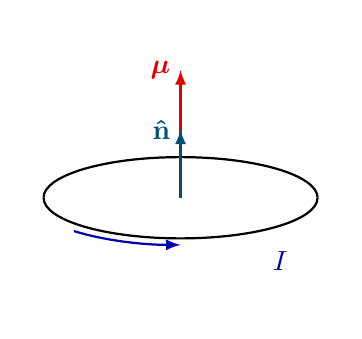
\begin{tikzpicture}[scale=1.2, thick]
  \def\Rx{1.45}
  \def\Ry{0.43}
  \def\h{0.5}
  \def\H{3}
  \def\L{4}
  \def\NB{5}
  \def\ang{36}
  \coordinate (O) at (0,0);
  \coordinate (N) at (0,0.24*\H);
  \coordinate (M) at (0,0.45*\H);
  \coordinate (B) at (\ang:\H);
  
  % MAGNETIC FIELD
  \draw (-\Rx,0) arc (180:0:{\Rx} and {\Ry});
  \begin{scope}
    \clip ({-0.5*\L*cos(\ang)},-0.4*\H) rectangle ++({\L*cos(\ang)},\H);
    %\foreach \i [evaluate={\y=(\i-0.5)*\H/(\NB-0.5)/2;
    %                       \yl=-\H/2+(\i-0.5)*\H/(\NB-0.5)/2;}] in {1,...,\NB}{
    %  %\draw[BFieldLine,thin] (0,\y)++(\ang-180:0.5*\L) --++ (\ang:\L);
    %  %\draw[BFieldLine,thin] (0,-\y)++(\ang-180:0.5*\L) --++ (\ang:\L);
    %  \draw[BFieldLine,thin] (-\H/2,\y) -- ({-\H/2+(\H/2-\y)*cos(\ang)},\H/2);
    %  \draw[BFieldLine,thin] (-\H/2,-\y) -- ({-\H/2+(\H/2+\y)*cos(\ang)},+\H/2);
    %  \draw[BFieldLine,thin] ({\H/2-(\H/2+\yl)*cos(\ang)},-\H/2) -- (\H/2,\yl);
    %  \draw[BFieldLine,thin] ({\H/2-(\H/2-\yl)*cos(\ang)},-\H/2) -- (\H/2,-\yl);
    %}
    % \foreach \i [evaluate={\x=-0.31*\H+(\i-1)*0.62*\H/(\NB-1);
    %                        \y=-cot(\ang)*\x;
    %                        \a=0.50+0.017*\i}] in {1,...,\NB}{ %0.58-0.02*(\i-\NB/2-1)^2
    %   \draw[BFieldLine=\a] (\x,\y)++(\ang-180:\H) --++ (\ang:2*\H);
      %\fill[red] (\x,\y) circle (0.05);
    % }
  \end{scope}
  % \node[Bcol] at (\H/2,0.49*\H) {$\vb{B}$};
  
  % CIRCUIT
  \draw[white,very thick]
        (-\Rx,0) arc (-180:0:{\Rx} and {\Ry});
  \draw (-\Rx,0) arc (-180:0:{\Rx} and {\Ry});
  %\draw[white,very thick] (0,0) ellipse ({\R} and {0.3*\R});
  %\draw (0,0) ellipse ({\R} and {0.3*\R});
  %\draw (0,0) ellipse ({\R} and {0.3*\R});
  \draw[mu vector] (0,0) -- (M) node[above=-1, left=0] {$\vb*{\mu}$};
  \draw[vector] (0,0) -- (N) node[below=0,left=0] {$\vu{n}$};
  % \draw pic[->,"\small$\;\theta$",draw=black,angle radius=14,angle eccentricity=1.4]
    % {angle = B--O--N};
  \draw[white,very thick]
    (-150:{1.1*\Rx} and {1.16*\Ry}) arc (-150:-80:{1.1*\Rx} and {1.16*\Ry});
  \draw[current]
    (-135:{1.1*\Rx} and {1.16*\Ry}) arc (-135:-90:{1.1*\Rx} and {1.16*\Ry})
    node[midway,right=2,below] {$I$};
  
\end{tikzpicture}


  \caption{Schematic of current loop and induced magnetic moment.}%
\end{wrapfigure}%


The \index{magnetic dipole}{magnetic dipole} produces a magnetic field $\vec{B}$, which for points a large distance from the dipole may be calculated as \cite{Griffiths2012-pt}:
\begin{equation}
    \vec{B} = \frac{\mu_0}{4\pi} \frac{1}{r^3} \left[\frac{3(\vec{\mu} \cdot \vec{r}) \cdot \vec{r}}{r^2} - \vec{\mu}\right]
    \label{eq:}
\end{equation}

The symmetry of the field enables us to consider the direction of the dipole as aligned to the $z$-axis. Then, defining $x,y$ as usual by $r \cos\theta$ and $r \sin\theta$ respectively. We may decompose the \index{magnetic field}{magnetic field} in two separate components, parallel ($B_z$) and perpendicular ($B_x, B_y$): 
$$B_\parallel =\frac{\mu_0}{r^3}(3\cos^2 \theta - 1), \quad B_\perp = \frac{3\mu_0}{r^3}\cos\theta\sin\theta.$$
Where we use the Pythagorean principle to determine the overall magnitude $B = |\vec{B}|$ as
$$B = \sqrt{B_\parallel^2 + B_\perp^2}.$$

\input{Sections/RabiOscillations.tex}
\subsection{Gyromagnetic Ratio}
\subsubsection{Classical Derivation}
The current in \eqref{eq:dipole_moment} is directly proportional to the current (i.e. the angular momentum of the charge). Specifically, we note that without angular momentum $\vec{G} = \vec{r} \times \vec{p}$ where $\vec{r}, \vec{p}$ represent the radius and the momentum respectively, the dipole moment would be zero.

Dividing the magnetic dipole moment by the angular momentum we find the \textbf{\index{gyromagnetic ratio}{gyromagnetic ratio}} \cite{Chen2020}
\begin{equation}
    \gamma = \frac{\vec{\mu}}{\vec{G}}.
    \label{eq:gyromagnetic_ratio}
\end{equation}

Without loss of generality we may consider the most simple case, in which the magnetic dipole moment is aligned with the angular momentum for which we may consider only the magnitudes of the dipole moment and the current (angular momentum)
\begin{equation}
    \mu = IS, \quad I = 
    % \underbrace{\frac{q}{2\pi R}}_{\rho \text{ (charge density)}}v,
    \frac{qv}{2\pi R},
    \quad S = \pi R^2 
    % \label{eq:}
\end{equation}
we substitute $I$ and $S$ to find 
\begin{equation}
    \mu = \frac{qvR}{2}
    % \label{eq:}
\end{equation}
% which we substitute into our equation for the gyromagnetic ratio 
% \begin{equation}
%     \gamma = \frac{\frac{qvR}{2}}{\vec{G}}. 
%     \label{eq:789}
% \end{equation}
and further, we equate the angular momentum vector, using the model of a planar loop to 
\begin{equation}
   G= m_q v R 
    % \label{eq:}
\end{equation}
leaving 
\begin{equation}
    \gamma = \frac{q}{2m_q } . 
    % \label{eq:}
\end{equation}

We finally consider that we may represent the, currently arbitrary, charge and mass as a sum of electron charges and masses. 
\begin{equation}
    \gamma = \frac{q}{2m_q } = \frac{\cancel{N}e}{2\cancel{N} m_e} \implies \gamma = \frac{e}{2 m_e}
    \label{eq:gyromagnetic_ratio_electrons}
\end{equation}

We therefore find that the gyromagnetic ratio of the electron depends only on fundamental constants \cite{bromley2000quantum}.

%pg 329 
% https://www.google.co.uk/books/edition/_/7qCMUfwoQcAC?hl=en&gbpv=1&bsq=walter%20greiner%20theoretical%20physics



\input{Sections/SpinInitialisation.tex}
\section{Lattice Symmetry}
Tetragonal lattice has the $$



\chapter{Task}
\section{Brief}

I think, as a start can go through section 3.2.4 in the attached PhD thesis? In particular check in details how to diagonalise the NV centre spin S=1 Hamiltonian to get Eq. 3.31?
You could also do some python simulations to plot how the spin levels (i.e. the eigenvalues of the spin Hamiltonian) change with applied magnetic field.

Once we've learned this, we can apply it to other spin defects in SiC.

\section{Work}
\subsection{Concepts and Nomenclature}
\subsubsection{Spin-Spin Interactions}
\subsubsection{Zeeman Splitting}
\subsubsection{Hyperfine Interaction}
\subsection{System Hamiltonian}\label{system_hamiltonian}
The ground state of the $\ce{NV^-}$ spin system in diamond is a triplet state, thus a $S=1$ system. 

The corresponding Hamiltonian, which it seems can be generalised to an electron spin system of a defect, can be expressed as: 
\begin{equation}
    H_{\ce{NV}} = H_{\ce{D}} + H_{\ce{Zeeman}} + H_{\ce{HF}} 
    \label{eq:nv_hamil}
\end{equation}

Here the labels $\ce{D}$, $\ce{Z}$ and $\ce{HF}$ describe the electron spin-spin interactions, the Zeeman interaction with an external magnetic field and the hyperfine interaction between the nuclparallel spin $I$ and the electron spin $S$ of the NV. 

They have the following forms: 
\begin{eqnarray}
    H_{\ce{D}} &=& D S_z^2 + E(S_x^2 + S_y^2) \label{H_D} \\
    H_{\ce{Z}} &=& g \mu_B \sum_{j}^{x,y,z} B_j \cdot S_j \label{H_Z} \\
    H_{\ce{HF}} &=& \vec{S} \cdot A \cdot \vec{I}. \label{H_HF}
\end{eqnarray}

\subsubsection{Spin-Spin Interaction}


The $E$ and $D$ in equation \ref{H_D} the fine structure constants of the spin
system, describing the spin-spin interaction and $S_j$ the corresponding spin operators
in x,y and z-direction. 

D is non-zero in system with axis of threefold (or other manifold) symmetry. 
The symmetry or spin quantization axis points along the connection of the nitrogen
atom and vacancy forming the defect. In bulk diamond $D$ is around 2.87 GHz at room temperature.

The definiteness, orientation and magnitude of $D$ is thus dependent on the specific spin system being studied. 

E occurs when there is a distortion of the point group symmetry, for example strain or an electrical field. In bulk diamond $E$ is typically negligibly small but especially in NDs, $E$ can be of the order of several MHz. 

Thus, similarly, the value of $E$ is a characteristic of the nature of the distortion and 
the specifics of the spin system being studied. 

\subsubsection{Zeeman Interaction}

$B_j$ in equation \ref{H_Z} is the magnetic field along the $x$, $y$ and $z$ direction, $g$ is the $g$-factor of the vacancy and $\mu_B$ the Bohr-Magneton, a constant. 

It seems often the scaled parameter $g\mu_B$ is considered, for the $\ce{NV^-}$ system this is around $28\;\ce{ GHz T^{-1}}$, but again, will be a characteristic of the system being studied. 

\subsubsection{Hyperfine Interaction}

Equation $\ref{H_HF}$ related the nuclear spin to the electron spin via the hyperfine tensor $A$ which has the form 
\begin{equation}
    A = \begin{pmatrix}
        A_\perp & 0 & 0 \\ 
        0 & A_\perp & 0 \\ 
        0 & 0 & A_\parallel
    \end{pmatrix}.
    \label{eq:hyperfine_tensor}
\end{equation}

$A_\parallel$ and $A_\perp$ are the axial and non-axial hyperfine parameters which encode two different interactions. 

\paragraph{Fermi Contact Interaction.}
This interaction is calculated by 
\begin{equation}
    f_A = \frac{A_\parallel + 2 A_\perp}{3}.
    \label{eq:fermi_contact}
\end{equation}

\paragraph{Anisotropic Interaction.}
This interaction is found by considering both spins as magnetic dipoles is calculated by 
\begin{equation}
    d_A = \frac{A_\parallel - A_\perp}{3}.
    \label{eq:anisotropic}
\end{equation}

For the $\ce{NV^-}$ system in diamond specifically, using the values for $A_\parallel$ and $A_\perp$ we calculate that $f_A$ is an order of magnitude stronger than $d_A$ for both $\ce{N^{14}}$ and $\ce{N^{15}}$. 

\subsubsection{Reduced Hamiltonian}
By combining $H_{\ce{D}}$ and $H_{\ce{Z}}$ 
and neglecting $H_{\ce{HF}}$ \todo{why (specifically) do we get to neglect this? Can we generalise?}
we find 
\begin{equation}
    H_{\ce{NV}} = D S_z^2 + E(S_x^2 + S_y^2) + g \mu_B \sum_{j}^{x,y,z} B_j \cdot S_j 
    \label{eq:reduced_H_NV}
\end{equation}

The spin operators $S_j$ in matrix representation are 
\begin{equation}
    S_x = \frac{1}{\sqrt{2}} \begin{pmatrix}
        0 & 1 & 0 \\ 
        1 & 0 & 1 \\ 
        0 & 1 & 0
    \end{pmatrix}, 
    S_y = \frac{i}{\sqrt{2}} \begin{pmatrix}
        0 & -1 & 0 \\ 
        1 & 0 & -1 \\ 
        0 & 1 & 0
    \end{pmatrix}, 
    S_z = \frac{1}{\sqrt{2}} \begin{pmatrix}
        1 & 0 & 0 \\ 
        0 & 0 & 0 \\ 
        0 & 0 & -1
    \end{pmatrix}. 
    \label{eq:spin_operators}
\end{equation}

Then, aligning the magnetic field (with strength $B_0$) along the $z$-axis (the quantisation axis), the reduced Hamiltonian will have the form 
\begin{equation}
    H_{\ce{NV}} = \begin{pmatrix}
        D + B_0 & 0 & E \\ 
        0 & 0 & 0 \\ 
        E & 0 & D-B_0
    \end{pmatrix},
    \label{eq:reduced_H_NV_matrix}
\end{equation}

with Eigenvalues 

\begin{equation}
    E_x = E_y = D \pm \sqrt{B_0^2  + E^2}, \; E_z = 0.
    \label{eq:reduced_H_NV_eigenvalues}
\end{equation}

The corresponding non-normalised Eigenvectors are then 

\begin{eqnarray}
    \ket{X} = \frac{1}{E} \left(B_0 + \sqrt{B_0^2 + E^2}\right) \ket{+1} + \ket{-1} \\ 
    \ket{Y} = \frac{1}{E} \left(B_0 - \sqrt{B_0^2 + E^2}\right) \ket{+1} + \ket{-1} \\ 
    \ket{Z} = \ket{0},
\end{eqnarray}
with
\begin{equation}
    \ket{1} = \begin{pmatrix}
        1 & 0 & 0 
    \end{pmatrix}, \; 
    \ket{0} = \begin{pmatrix}
        0 & 1 & 0 
    \end{pmatrix}\;, 
    \ket{-1} = \begin{pmatrix}
        0 & 0 & 1 
    \end{pmatrix},
    \label{eq:base_states}
\end{equation}
the Eigenvectors for $H_{\ce{NV}}$ with $E=0$\dots

In the case where $E \ll B_0$ the Eigenvectors are well described by the bases $\ket{0}$ and $\ket{\pm 1}$.

For $E \gg B_0$, when transforming the spin operators $S_j$ into the diagonalised system with Hamiltonian $H_{\ce{NV}}$ they read 
\begin{equation}
    \hat{S}_x^\parallel \propto \begin{pmatrix}
        0 & 1 & 0 \\ 
        1 & 0 & 0 \\ 
        0 & 0 & 0 
    \end{pmatrix} \; , 
    \hat{S}_y^\parallel \propto \begin{pmatrix}
        0 & 0 & 0 \\ 
        0 & 0 & -i \\ 
        0 & i & 0 
    \end{pmatrix} \; , 
    \hat{S}_z \propto \begin{pmatrix}
        0 & 0 & -1 \\ 
        0 & 0 & 0 \\ 
        -1 & 0 & 0 
    \end{pmatrix} , 
    \label{eq:diagonalised_spin_operators}
\end{equation}
and 
\begin{equation}
    \hat{H}_{\ce{NV}} = \begin{pmatrix}
        D + \sqrt{B_0^2 + E^2} & 0 & 0 \\ 
        0 & 0 & 0 \\ 
        0 & 0 & D - \sqrt{B_0^2 - E^2}. 
    \end{pmatrix} 
\end{equation}

Another solution for a $\pi/2$ shifted, modulating magnetic field leads to 
\begin{equation}
    \hat{S}_x^\perp \propto \begin{pmatrix}
        0 & 0 & 0 \\ 
        0 & 0 & 1 \\ 
        0 & 1 & 0 
    \end{pmatrix} \; , 
    \hat{S}_y^\perp \propto \begin{pmatrix}
        0 & -i & 0 \\ 
        i & 0 & 0 \\ 
        0 & 0 & 0 
    \end{pmatrix} \; , 
    \hat{S}_z \propto \begin{pmatrix}
        0 & 0 & 1 \\ 
        0 & 0 & 0 \\ 
        1 & 0 & 0 
    \end{pmatrix} , 
    \label{eq:diagonalised_spin_operators}
\end{equation}
a physical interpretation of which is that a linear modulating B-field aligned
along the $x$-axis where strain is applied only allows transitions between the state
$\ket{X}$ and $\ket{0}$, whereas fields perpendicular to the strain and the NV quantization axis
only allow coupling between $\ket{Y}$ and $\ket{0}$.

For an arbitrary external magnetic field, $H_\ce{NV}$ can be expressed using spherical co-ordinates: 
\begin{equation}
    H_{\ce{NV}} = \begin{pmatrix}
        D + B_0 \cdot \cos \theta & \frac{B_0}{\sqrt{2}} \cdot e^{-i\cdot \varphi} \cdot \sin\theta & E \\ 
        \frac{B_0}{\sqrt{2}} \cdot e^{i \cdot \varphi} \cdot \sin\theta & 0 & \frac{B_0}{\sqrt{2}} e^{-i\cdot \varphi} \cdot \sin\theta \\ 
        E & \frac{B_0}{\sqrt{2}} \cdot e^{i \cdot \varphi} \cdot \sin\theta & D - B_0 \cdot \cos \theta
    \end{pmatrix}
    \label{eq:nv_hamil_spherical_matrix}
\end{equation}


Here, we transformed the magnitude of the arbitrary magnetic field into spherical co-ordinates as 
\begin{eqnarray}
    B_x  &=& B_0 \cos\varphi \sin\theta \\ 
    B_y  &=& B_0 \sin\varphi \sin\theta \\ 
    B_z  &=& B_0 \cos\theta 
\end{eqnarray}
with $\theta$ the azimuthal and $\varphi$ the polar angle. Then using equations \ref{eq:reduced_H_NV} and \ref{eq:spin_operators} we compute \ref{eq:nv_hamil_spherical_matrix}.  

It immediately follows from the characteristic equation that Eigenvalues $\lambda$ satisfy 
\begin{equation}
    0 = \lambda^3 - 2\cdot \lambda^2 \cdot D + \frac{D \cdot B_0^2}{2} + \lambda(D^2 - E^2 - B_0^2) - \frac{1}{2}B_0^2\underbrace{\left(D \cdot \cos(2\theta) - 2 \cdot E \cos(2\varphi) \cdot \sin(\theta)^2\right)}_{\Delta_{\varphi \theta}}
    \label{eq:nv_spherical_characteristic_equation}
\end{equation}
% \cite{balasubramanian2009}





\chapter{Design}
In this chapter we will provide an overview of how the defects in SiC can be used for magnetometry, thermometry and electrometry in isolation. We will then develop a framework where by combining specific defects we may simultaneously measure multiple parameters. 

\section{$S=1$ Magnetometry}
We begin by considering a triplet state, that is a $S=1$ system. 

Under the influence of a magnetic field, the Hamiltonian can be expressed as: 
\begin{equation}
    H_{} = H_{\ce{D}} + H_{\ce{Z}}} 
    \label{eq:nv_hamil}
\end{equation}

Here the labels $\ce{D}$ and $\ce{Z}$ describe the electron spin-spin interactions and the Zeeman interaction with an external magnetic field. 

They have the following forms: 
\begin{eqnarray}
    H_{\ce{D}} &=& D S_z^2 + E(S_x^2 + S_y^2) \label{H_D} \\
    H_{\ce{Z}} &=& g \mu_B \sum_{j}^{x,y,z} B_j \cdot S_j \label{H_Z} \\
\end{eqnarray}

\subsubsection{Spin-Spin Interaction}

The $E$ and $D$ in equation \ref{H_D} represent the fine structure constants of the spin
system, describing the spin-spin interaction and $S_j$ the corresponding spin operators
in x,y and z-direction. 

$D$ is non-zero in system with axis of threefold (or other manifold) symmetry. 
The definiteness, orientation and magnitude of $D$ is dependent on the specific spin system being studied. 

$E$ occurs when there is a distortion of the point group symmetry, for example strain or an $\vec{E}$ field. 
Similarly, the value of $E$ is a characteristic of the nature of the distortion and 
the specifics of the spin system being studied. 

\subsubsection{Zeeman Interaction}

$B_j$ in equation \ref{H_Z} is the magnetic field along the $x$, $y$ and $z$ direction, $g$ is the $g$-factor of the vacancy and $\mu_B$ the Bohr-Magneton. 

% It seems often the scaled parameter $g\mu_B$ is considered, for the $\ce{NV^-}$ system this is around $28\;\ce{ GHz T^{-1}}$, but again, will be a characteristic of the system being studied. 

% \subsubsection{Reduced Hamiltonian}
By combining $H_{\ce{D}}$ and $H_{\ce{Z}}$ 
we find 
\begin{equation}
    H_{} = D S_z^2 + E(S_x^2 + S_y^2) + g \mu_B \sum_{j}^{x,y,z} B_j \cdot S_j 
    \label{eq:reduced_H_NV}
\end{equation}

The $S=1$ spin operators $S_j$ in matrix representation are 
\begin{equation}
    S_x = \frac{1}{\sqrt{2}} \begin{pmatrix}
        0 & 1 & 0 \\ 
        1 & 0 & 1 \\ 
        0 & 1 & 0
    \end{pmatrix}, 
    S_y = \frac{i}{\sqrt{2}} \begin{pmatrix}
        0 & -1 & 0 \\ 
        1 & 0 & -1 \\ 
        0 & 1 & 0
    \end{pmatrix}, 
    S_z = \frac{1}{\sqrt{2}} \begin{pmatrix}
        1 & 0 & 0 \\ 
        0 & 0 & 0 \\ 
        0 & 0 & -1
    \end{pmatrix}. 
    \label{eq:spin_operators}
\end{equation}

Then, aligning the magnetic field (with strength $B_0$) along the $z$-axis (the quantisation axis), the reduced Hamiltonian will have the form 
\begin{equation}
    H_{} = \begin{pmatrix}
        D + B_0 & 0 & E \\ 
        0 & 0 & 0 \\ 
        E & 0 & D-B_0
    \end{pmatrix},
    \label{eq:reduced_H_NV_matrix}
\end{equation}

with Eigenvalues 

\begin{equation}
    E_x = E_y = D \pm \sqrt{B_0^2  + E^2}, \; E_z = 0.
    \label{eq:reduced_H_NV_eigenvalues}
\end{equation}

The corresponding non-normalised Eigenvectors are then 

\begin{eqnarray}
    \ket{X} = \frac{1}{E} \left(B_0 + \sqrt{B_0^2 + E^2}\right) \ket{+1} + \ket{-1} \\ 
    \ket{Y} = \frac{1}{E} \left(B_0 - \sqrt{B_0^2 + E^2}\right) \ket{+1} + \ket{-1} \\ 
    \ket{Z} = \ket{0},
\end{eqnarray}
with
\begin{equation}
    \ket{1} = \begin{pmatrix}
        1 & 0 & 0 
    \end{pmatrix}, \; 
    \ket{0} = \begin{pmatrix}
        0 & 1 & 0 
    \end{pmatrix}\;, 
    \ket{-1} = \begin{pmatrix}
        0 & 0 & 1 
    \end{pmatrix},
    \label{eq:base_states}
\end{equation}
the Eigenvectors for $H$ with $E=0$ \td{Need to finish write up. }.

In the case where $E \ll B_0$ the Eigenvectors are well described by the bases $\ket{0}$ and $\ket{\pm 1}$.

For an arbitrary external magnetic field, $H$ can be expressed using spherical co-ordinates: 
\begin{equation}
    H = \begin{pmatrix}
        D + B_0 \cdot \cos \theta & \frac{B_0}{\sqrt{2}} \cdot e^{-i\cdot \varphi} \cdot \sin\theta & E \\ 
        \frac{B_0}{\sqrt{2}} \cdot e^{i \cdot \varphi} \cdot \sin\theta & 0 & \frac{B_0}{\sqrt{2}} e^{-i\cdot \varphi} \cdot \sin\theta \\ 
        E & \frac{B_0}{\sqrt{2}} \cdot e^{i \cdot \varphi} \cdot \sin\theta & D - B_0 \cdot \cos \theta
    \end{pmatrix}
    \label{eq:nv_hamil_spherical_matrix}
\end{equation}


Here, we transformed the magnitude of the arbitrary magnetic field into spherical co-ordinates as 
\begin{eqnarray}
    B_x  &=& B_0 \cos\varphi \sin\theta \\ 
    B_y  &=& B_0 \sin\varphi \sin\theta \\ 
    B_z  &=& B_0 \cos\theta 
\end{eqnarray}
with $\theta$ the azimuthal and $\varphi$ the polar angle. Then using equations \ref{eq:reduced_H_NV} and \ref{eq:spin_operators} we compute \ref{eq:nv_hamil_spherical_matrix}.  

It immediately follows from the characteristic \td{need to finish writing this} equation that Eigenvalues $\lambda$ satisfy 
\begin{equation}
    0 = \lambda^3 - 2\cdot \lambda^2 \cdot D + \frac{D \cdot B_0^2}{2} + \lambda(D^2 - E^2 - B_0^2) - \frac{1}{2}B_0^2\underbrace{\left(D \cdot \cos(2\theta) - 2 \cdot E \cos(2\varphi) \cdot \sin(\theta)^2\right)}_{\Delta_{\varphi \theta}}
    \label{eq:nv_spherical_characteristic_equation}
\end{equation}
% \cite{balasubramanian2009}




% https://magnetometryrp.quantumtinkerer.tudelft.nl/3_NVspin/


\subsection{$\vec{B}$ Parallel to Defect Axis}
The simplest implementation of the magnetometer is when the applied magnetic field, $B_0$ is parallel to the defect axis. 

In this case, the entire magnitude of the field contributes to the Zeeman splitting of the energy level. This means in the CW-ODMR spectra the difference between the two frequencies $f_1 > f_2$ is directly proportional to $B_0$ and related as detailed in Section \ref{zeeman}.
$$f_1 = D + \gamma B_0,  \quad f_2 = D - \gamma B_0$$
It is then straightforward to calculate $B_0$ using 
$$B_0 = \frac{f_1 - f_2}{2 \gamma} $$
which is visualised for the DNV system in figure \ref{fig:spin1_magnetometry}. 

\begin{figure}[h]
    \begin{center}
    \includegraphics[width=0.7\textwidth]{figures/NVlevelwithESR.png}
% \missingfigure{Two panel figure. Panel 1 - energy level splitting of S=1 system being prop to gyromagnetic ratio. Panel 2 - ODMR Spectra} 
    \end{center}
    \caption{Magnetometry with $\theta = 0$. Left shows the lifting of degeneracy of the spin system energy levels with the applied $\vec{B}$ field. Right shows the corresponding ODMR spectra and two EPR frequencies \cite{dnvweb}. }
\label{fig:spin1_magnetometry}
\end{figure}


\subsubsection{$\vec{B}$ at Angle $\theta$ to Defect Axis}
The Zeeman effect is proportional to $\cos\theta$, thus, when $\vec{B}$ is perpendicular to the defect axis the Zeeman effect reduces to zero, varying the azimuthal angle $\theta$ is effectively the same as scaling $B_0$ by $\cos \theta$. 

\begin{figure}[h]
    \begin{center}
 % /        \missingfigure{ODMR or Energy Eigenvalues plot for $\theta = 0, 30, 60, 90$ showing the effective reduction of applied parallel field.}
    \includegraphics[width=0.95\textwidth]{figures/PL6ODMRSpectra_theta_0_to_90.png}
    \end{center}
    \caption{ODMR/Energy level plot showing the reduction of the effective parallel $\vec{B}$ field with increasing $\theta$.} 
    \label{fig:}
\end{figure}


\subsection{$S=1$ Vector Magnetometry}
Vector magnetometry with a $S=1$ system can be achieved by comparing the relative intensities from defects known to be at specific angles. 

For example, in diamond the nitrogen vacancy is aligned with the tetragonal crystal structure and thus may take one of four orientations as illustrated in Figure \ref{fig:dnv_orientations}. 

\begin{figure}[h]
    \begin{center}
        % \missingfigure{Sketch of DNV and possible defect orientations.}
        \includegraphics[width=0.45\textwidth]{figures/four_possible_NV_orientations.png}
    \end{center}
    \caption{Diagram showing the four possible orientations of NV centers in diamond \cite{pham}.}\label{fig:dnv_orientations}
\end{figure}


The 4 possible DNV orientations in the lattice are $111$, $1\overline{11}$, $\overline{1}1\overline{1}$ and $\overline{11}1$. 
Once the projections of the magnetic field along these axes have been measures, we reconstruct the magnetic field in the laboratory frame.

The ODMR sprectrum for a sample of diamond with approximately equal distribution of the four defect orientations. 

% # file:///home/conner/Downloads/e2015-60080-1.pdf
\td{Finish typing - link in comments}
The measured field components $m_i$ do not directly give the magnetic field $B_i$, but are affected by some noise in-
herent to the measurement which is accounted for using a maximum-likelihood method. 

\lipsum[1-6]
% The direction of $\vec{B}$ relative to the crystal lattice can then be determined by solving 
% \begin{equation}
%     \underbrace{
%     \frac{1}{\sqrt{3}}
%     \begin{pmatrix}        
%         1 & 1 & 1 \\ 
%         -1 & -1 & 1 \\ 
%         -1 & 1 & -1 \\ 
%         1 & -1 & -1 
% \end{pmatrix}}_{N}
%     \mathbf{\hat{B}} = 
%     \underbrace{
%     \begin{pmatrix}
%         \cos\theta_1 \\
%         \cos\theta_2 \\
%         \cos\theta_3 \\
%         \cos\theta_4 \\
%     \end{pmatrix}
% }_{\mathbf{c}}
%     \label{eq:}
% \end{equation}
% For which a solution may be determined 
% \begin{equation}
%     \mathbf{\hat{B}} = \left(N^T N\right)^{-1} N^T \mathbf{c}.   
%     \label{eq:}
% \end{equation}
%
% With knowledge of .. \td{Need to finish writing about knowing the miller index family of crystal can convert miller vector to lab vector}. 
%

\cite{Balasubramanian2008}
\td{Need to also look at this method and type up}

\section{$S = 3/2$ Magnetometry}
% V2 
\cite{PhysRevApplied.4.014009}
\cite{PhysRevB.92.115201}
\cite{1505.06914}

If the ZFS interaction of the $S=3/2$ defect is sufficiently strong, the eigenvalues of the
spin Hamiltonian show a strong dependence on the orientation of the applied magnetic field. 

This induces a non-linear shift of resonance transitions in EPR frequencies, which is seen in the ODMR spectra. 
This allows information about the applied external magnetic field to be extracted from ESR spectra provided the ZFS is known. 

In zero magnetic field the $V_{\ce{Si}}$ V2 vacancy has an ODMR line maximum around 70 MHz with very weak dependence on temperature. That is, the ZFS parameter is known and resistant to the environmental influence of temperature. 

In a $S=3/2$ spin system the orientation related terms are, like for $S=1$ systems, in the eigenvalue equation. 
This results in the orientation dependent shift of EPR frequencies which are not explained by $g \mu_B B_0$ as they are for $S=1$. 

Therefore in order to reconstruct the energy eigenstates we must use the observed resonant energies. There are $2S +1 $ states for a system with spin $S$ from which $2S$ transition frequencies may be found. 


% Applying a magnetic field $B_0$ along the defect axis, $\theta = 0$, 

For the V2 $V_{\ce{Si}}$, $E \ll D$ and a uniaxial symmetry exists therefore the Hamiltonian for the system is given as in equation \ref{}\td{ref correct hamiltonian}. Here we use the 4-dimensional $S=3/2$ matrix representation 
\begin{equation}
    \label{eq:}
\end{equation}
    \td{Add spin 3/2 matrices} 

    For this defect, using the same polar co-ordinate conversion as in section \ref{}\td{find ref} we may write the Hamiltionian in matrix form \td{Add hamiltonian matrix} and find the eigenvalue equation 
\begin{equation}
    \begin{align}
    &\lambda^4 - \left(2D^2 + 6E^2  + \frac{5}{2}(g\mu_B B_0)^2 \right)\lambda^2 - 2 (g \mu_B B_0)^2 \left(D(3 \cos^2 \theta -1) + 3E \sin^2\theta \cos 2\varphi \right)\lambda \\ 
    &+\frac{9}{16}(g \mu_B B_0)^4 + D^4 - \frac{1}{2}D^2 (g \mu_B B_0)^2 - D^2 (g \mu_B B_0)^2 (3 \cos^2 \theta - 1) + 3E^2(3E^2 + 2D^2) \\ 
    &+ E(g\mu_BB_0)^2 (6D \sin^2\theta \cos 2\varphi + \frac{9}{2}E \cos2\theta) = 0 
    \end{align} 
    \label{eq:V2_eigenvalue_equation}
\end{equation}
 
Considering $B_0$ componentwise we may find \cite{Kirmse1995} for $B_0$ parallel to the defect axis 
\begin{equation}
\lambda = \frac{1}{2}g\mu_B B_0 \pm \sqrt{(D + g\mu_B B_0)^2 + 3E^2} 
   \text{ or, }
   \lambda = -\frac{1}{2} g\mu_B B_0 \pm \sqrt{(D-g\mu_B B_0)^2 + 3E^2}.
    % \label{eq:}
\end{equation}

For $B_0$ perpendicular to the defect axis we find:
\begin{equation}
    \begin{align}
        &\lambda = \frac{1}{2}g\mu_B B_0 \pm \sqrt{(g\mu_B B_0)^2 + D^2  + 3E^2 - (D - 3E)g\mu_B B_0}\text{ or, }\\
        \lambda &= -\frac{1}{2}g\mu_B B_0 \pm \sqrt{(g\mu_B B_0)^2 + D^2 + 3E^2 + (D-3E)g\mu_B B_0}.
    \end{align}
\end{equation}

We may write the general equation for the eigenvalues as 
\begin{equation}
    \sum_{n=0}^{2S+1} C_n \lambda^n = 0
    \label{eq:}
\end{equation}
we then substitute each eigenvalue $\lambda_i$ into this general expression to obtain $2S + 1$ equations. 

The goal is now to remove all $\lambda_i$ terms by considering instead the transition frequencies between eigenstates, which are observed in the ODMR spectra. The energy states are not in general sorted with respect to the energy values, so we use the convention that $\lambda_i > \lambda_{i-1}$. 

To reduce our number of equations to $2S-1$ we make the substitutions  
$$\lambda_i + \underbrace{\lambda_{i+1} - \lambda_{i}}_{f_{i+1, i}} = \lambda_{i+1},
\qquad\lambda_i - \underbrace{(\lambda_{i} - \lambda_{i-1})}_{f_{i, i-1}} = \lambda_{i-1}$$
for each $i = 2, \dots, 2S$ and calculate both 
$$\sum_{n=0}^{2S +1} \frac{C_n \left((\lambda_i + f_{i+1, i})^n - \lambda_i^n\right)}{C_{2S+1}} = 0\text{ and } \sum_{n=0}^{2S +1}\frac{C_n \left((\lambda_i - f_{i, i-1})^n - \lambda_i^n\right)}{C_{2S + 1}} = 0$$
to find two new simultaneous equations 
$$\sum_{n=0}^{2S} C_{i,n}' \lambda_i^n = 0 \text{ and } \sum_{n=0}^{2S} C''_{i,n}\lambda_i^n = 0.$$

We may combine these as 
$$\sum_{n=0}^{2S} \frac{C'_{i,n}\lambda_i^n}{C'_{i,2S}}-\frac{C''_{i,n} \lambda_i^n}{C''_{i, 2S}} = 0$$
to obtain an equation for the eigenvalue of the energy eigenstate $\ket{i}$ where $i = 2, \dots, 2S$: 

\begin{equation}
    \sum_{n=0}^{2S -1} C_{i,n}^{(2S-1)} \lambda_i^n = 0.
    \label{eq:refmenowpls}
\end{equation}

This process is repeated until only one linear equation exists for each eigenvalue, which may be expressed in terms of resonant energies. $f_{i, i-1}$ can then be substituted to find expressions for all other eigenvalues. 

For the V2 $V_{\ce{Si}}$, we obtain equations for $\lambda_2$ expressed in terms of $f_{2,1}, f_{3,2}$ and $\lambda_3$ expressed in terms of $f_{3,2}, f_{4,3}$. Finally, using $f_{3,2} = \lambda_3 - \lambda_2$ we find formulas for each eigenvalues in terms of the resonant frequencies: 

\begin{eqnarray}
    \lambda_1 = -\frac{3}{4}f_{2,1} - \frac{1}{2} f_{3,2} - \frac{1}{4} f_{4,3}\\ 
    \lambda_2 = \frac{1}{4}f_{2,1} - \frac{1}{2}f_{3,2} - \frac{1}{4} f_{4,3} \\ 
    \lambda_3 = \frac{1}{4}f_{2,1} + \frac{1}{2}f_{3,2} - \frac{1}{4} f_{4,3} \\ 
    \lambda_4 = \frac{1}{4}f_{2,1} + \frac{1}{2}f_{3,2} + \frac{1}{4} f_{4,3}.
\end{eqnarray}

We substitute one of these expressions into one of the equations of the form of equation \ref{eq:refmenowpls} and we obtain 
\begin{equation}
    \begin{align}
        5(g\mu_B B_0)^2 &=\left(\frac{\sqrt{3}}{2}f_{4,3} + f_{3,2}  + \frac{\sqrt{3}}{2}f_{2,1}\right)^2 \\ 
        &+(1 - \sqrt{3}) (f_{4,3} + f_{2,1})f_{3,2} - f_{4,3}f_{2,1} - 4(D^2 + 3E^2).
    \end{align}
    \label{eq:V2_magnitude}
\end{equation}

A second quantity $\eta$, useful for angle resolution (next section) related to the polar and azimuthal angle is also defined

\begin{equation}
        \eta \equiv E(2\cos^2\varphi \sin^2 \theta + \cos^2\theta) + D\cos^2 \theta 
    \label{eq:eta}
\end{equation}

which in terms of the resonant frequencies is given by 
\begin{equation}
    \begin{align}
    &\eta = \\ 
    &\frac{4\left(8(D + 3E) + 5(f_{4,3}-f_{2,1})\right)(g\mu_B B_0)^2 + (f_{4,3} - f_{2,1})\left(16(D^2 + 3E^2) - (f_{4,3}-f_{2,1})^2 - 4f_{3,2}^2\right)}{96(g\mu_B B_0)^2}
\end{align}
    \label{eq:eta_resonant}

\end{equation}


Overall, this shows that if the ZFS is known and three EPR frequencies are observes, the applied magnetic field strength can be found using equation \ref{eq:V2_magnitude}


% \subsection{$\vec{B}$ Parallel to Defect Axis}

% The simplest possible cashen $\theta = 0$ there is no super-position of states and selection rules dictate that the only transitions available 

\subsection{$S=3/2$ Angle Resolved Magnetometry}
We may approximate $\eta$ defined in equation \ref{eq:eta} for the V2 $V_{\ce{Si}}$, which exhibits uniaxial symmetry, i,e, $E\ll D$, to 
\begin{equation}
    \eta \sim D \cos^2 \theta. 
    \label{eq:}
\end{equation}

By exploiting this approximation, we may also determine the polar angle that the magnetic field vector makes with the defect axis, however at this stage we may not determine anything about the $x,y$ components of the vector. 

To do so we explicitly compute $\eta$ using equation \ref{eq:eta_resonant} then we find the polar angle as 
\begin{equation}
    \theta = \cos^{-1}\sqrt{\frac{\eta}{D}}
    \label{eq:vector_theta}
\end{equation}


\subsection{$S = 3/2$ Vector Magnetometry}
Vector magnetometry is achieved in the case of the DNV as described in section \ref{dnv_vector} \td{link reference} and theoretically a similar approach is possible in SiC. There exists two distinct and differently oriented Silicon vacancies in 4H-SiC and three in 6H-SiC \cite{Janzn2009}. In practice however, in practice at least one of the defects in each polytope is difficult to observe at room temperature making this approach unsuitable for vector magnetometry. 

In a general $S = 3/2$ system, ambiguity is found when computing $\theta$ using equation \ref{eq:vector_theta} as the EPR frequencies can not be mapped to specific transitions. 

The following approach exploits the fact that a crossing of resonant frequencies occurs at a given angle (see figure \ref{fig:resonant_crossing_V2}). The method should be considered for $g\mu_B B_0 \gg 2\sqrt{D^2 + 3E^2}$ explicitly as interactions such as level anti-crossing produce a complex spectra \cite{Degen2008} when $g\mu_B B_0 \approx 2\sqrt{D^2 + 3E^2}$ and the invariance of a particular EPR frequency when $g \mu_B B_0 \ll 2 \sqrt{D^2 + 3E^2}$ makes determination of the polar angle $\theta$ impossible. 

\begin{figure}[h]
    \begin{center}
        % \includegraphics[width=0.95\textwidth]{figures/}
        \missingfigure{Plot showing the crossing of EPR frequencies at high field and low field in Spin 3/2 system as theta varies}
    \end{center}
    \caption{}\label{fig:resonant_crossing_V2}
\end{figure}
\begin{group}
    \color{gray}
At a high B0 field (gμB B0  ZFS),
B0 can be obtained from the observed ESR spectra but
the polar angle cannot be determined due to the ambigu-
ity of differentiating two outer transitions. In contrast,
at low gμB B0 ( ZFS), as long as one can explicitly
identify at least three transitions including the allowed
lowest energy transition, the external magnetic field vec-
tor can be reconstructed. In the field strength compara-
ble to the ZFS, it is hard to find a useful scheme because
very complex patterns appear due to mixing of some of
the eigenstates. In the case of the NV centers in dia-
mond (ZFS/h=2.87 GHz), this missing range is around
∼ 100 mT . The VSi in SiC can fill out this gap since its
ZFS is quite small (ZFS/h ∼ 100 MHz) thus this mag-
netic field range can be considered as a high field range
in which the three necessary transitions are well observ-
able25,29, and at least the field strength can be experi-
mentally determined. When the VSi in SiC is used to
realize such schemes at sub-mT, if the lowest transition
energy is observable by ELDOR, one can determine both
B0 and θ without ambiguity. 
% Even if ELDOR is not avail-
% able, thanks to the additional transitions that appear at
% low fields, the field strength can be determined.
% The magic angle terms in the eigenvalue equation al-
% low for an alternative method to use S=3/2 systems as
% a DC vector magnetometer. If the S=3/2 spins fixed
% in a crystal can be rotated around the rotational axis,
% the unambiguous determination of the applied magnetic
% field vector is feasible by monitoring the linewidth of the
% observed ESR spectra while the symmetry axis of the
% crystal is oriented at θm relative to the rotational axis
% and the rotational axis is moving. This configuration
% also can be realized by producing an array of the crystals
% such that the symmetry axes of each crystal form a cone
% whose opening angle is twice the magic angle.
% These findings provide a better understanding of the
% S=3/2 electronic spin Hamiltonian, especially at low
% fields. They also provide an outlook for the application of
% VSi in SiC to quantum magnetometry which is promising
% thanks to the electrical properties of SiC, which outstand
% the host material of the NV centers, and the mature fab-
% rication technology, which allows an efficient fabrication
% of electronic devices even at the atomic scale48
\end{group}


 % In addition, it is demonstrated that the observation of the central line of the TV2a center of S = 3/2 has been achieved by pulsed-ELDOR
\cite{Isoya2008}


% \cite{Kraus2014}

\section{Sensing Pressure*}
\cite{doi:10.1021/acs.nanolett.2c03378}
\cite{PhysRevLett.112.087601}
\cite{PhysRevLett.112.187601}

\section{$S=1$ Thermometry}
\cite{Chen2011}
\cite{ajev2009}
\cite{PhysRevApplied.8.044015}
\cite{D3NR00430A}
\cite{PhysRevApplied.10.044042}
\cite{PhysRevB.104.125305}
\cite{PhysRevB.91.155404}

% Example
\cite{Quan:23}

\tdr{Distribute references properly}


We can use spin defects in SiC for temperature sensing. 
There are two main approaches to thermometry:
\begin{description}
    \item[ZFS Temperature Dependence.] The ZFS parameters $D$ and $E$ may, depending on the specific spin system being studies, be sensitive to changes in temperature. 
    \item[Photoluminescence.] The photoluminescence of the spin system may have a dependence on temperature. 
\end{description}

This work will focus on the first method of thermometry. Unlike $\vec{B}$ and $\vec{E}$ field sensing, there is no direction associated with temperature so the sensing regime may be simpler.  

For SiC divacancies, which are triplet states, the ZFS parameter $E$ shows no dependence on temperature. However, the ZFS parameter $D$ varies with temperature. 

The value of $D$ for both the PL5 and PL6 defects in SiC has been measured from close to $0$K to around $550$K and the dependence of $D$ has been fitted to the change in temperature. 
Both defects show an approximately linear relationship near room temperature which is shown in Figure \ref{fig:PL5PL6DvsT}

\begin{figure}[h]
    \begin{center}
    % \missingfigure{Plot of both the PL5 and PL6 temperature dependence from 0 to 550K, specifically highlighting the linear region. }
    \includegraphics[width=0.49\textwidth]{figures/SiC-PL5PL6-D(T).png}
    \includegraphics[width=0.49\textwidth]{figures/SiC-PL5PL6-D(T)-close.png}
    \caption{ZFS parameter $D$ temperature dependence for the PL5 and PL6 $S=1$ defect in SiC from 0-550 K (left) and 250-350 K (right). }\label{fig:PL5PL6DvsT}
\end{center}
\end{figure}

\td{Update the T dependence of PL5 and PL6 and regen the figure. Also update temp linear range in figure caption.}

In the simplest case thermometry is then achieved in the presence of a well known applied magnetic field. 

The measurement stems from the change of the value of
D mapped into the change of the oscillation frequency of the
relative variation of the photoluminescence intensity induced by the microwave pulse sequence.

Since the degeneracy is raised symmetrically, the value of $D$ is the average of the two resonant frequencies. The value of $D$ can then be mapped to a temperature. 

This is visualised in figure \ref{fig:pl6-3temps}. 

\begin{figure}[h]
    \begin{center}
        \includegraphics[width=0.8\textwidth]{figures/PL6-DvsT-3temps.png}
    \end{center}
    \caption{}\label{fig:pl6-3temps}
\end{figure}

In practice this \td{Write up the Ramsey Interference methods for c-axis and basal from Castello p18}. 
\lipsum[1]

\section{$S= 3/2$ Thermometry}
\lipsum[3-5]

\section{$S = 1$ Electometry}
\todo[inline]{Add matrix Hamiltonian as well as eigenval solutions. Include the formula for $\Delta \omega$ and dicuss the diminishing returns when $B\neq0$ or if $B \not\perp z$}

\section{$S=3/2$ Electrometry}

\section{Sensing Strain*}
\lipsum[1-3]
\td{Strain and applied $\vec{E}$ field are indistinguishable so can use $E$ techniques in shielded environment to determine strain.}


\section{Multimodality}
To develop our multimodal system we will start with a very simple model with the assumption that the applied $\vec{B}$ field is parallel to the defect axis. From there we will iterate our ensemble and work to reduce the number of assumptions.  


\subsection{$|\vec{B}|$ and $T$}
\cite{Degen2008}
\lipsum[1-4]

\subsection{Angle Resolved $|\vec{B}|$ and $T$}
% We show that uniaxial color centers in silicon carbide with hexagonal lattice structure can be used to measure not only the strength but also the polar angle of the external magnetic field with respect to the defect axis with high precision. 
\cite{PhysRevApplied.4.014009}
\lipsum[1-4]

\subsection{$\vec{B}$ and $T$}
\lipsum[1-4]


\subsection{$|\vec{B}|$, $|\vec{E}|$ and $T$}
The influence of an $\vec{E}$ field parallel to the defect axis is indistinguishable from the influence of a change of temperature. Similarly, the influence of an $\vec{E}$ field perpendicular to the defect axis is indistinguishable from the influence of a $\vec{B}$ field parallel to the defect axis. The exception is when \td{When $B_0$ is smaller than ZFS E when the effects can be distinguished}... 

\begin{figure}[h]
    \begin{center}
        % \includegraphics[width=0.95\textwidth]{figures/}
        \missingfigure{2 plots. Both of a basline energy graph and showing the similarity of T and parallel E, and B and perp E.}
    \end{center}
    \caption{}\label{fig:}
\end{figure}


Thus, to extend the multi-modality to include the $\vec{E}$ field we must isolate the influence of the $\vec{E}$ field from the other environmental factors. 


\lipsum[1-4]

\subsection{$\vec{B}$, $\vec{E}$ and $T$}
\lipsum[1-8]
%
% This section should be written in standard scientific
% language. Standard techniques in your research field should not be
% written out in detail. In computational projects this section should
% be used to explain the algorithms used and the layout of the
% computational code. A copy of the actual code may be given in the
% appendices if appropriate.
%
% This section should emphasise the philosophy of the approach used and
% detail novel techniques. However please note: this section should not
% be a blow-by-blow account of what you did throughout the project. It
% should not contain large detailed sections about things you tried and
% found to be completely wrong! However, if you find that a technique
% that was expected to work failed, that is a valid result and should be
% included.
%
% Here logical structure is particularly important, and you may find
% that to maintain good structure you may have to present the
% explorations/calculations/computations/whatever in a different order
% from the one in which you carried them out.
%
%
% You might sometimes want to include multiple equations in one place
% \begin{eqnarray}
%   E &=& ma^{2} \\
%   E &=& mb^{2} \\
%   E &=& mc^{2}
% \end{eqnarray}
% You might want to include multiple equations in one place without
% numbering them
% \begin{eqnarray*}
%   E &=& ma^{2} \\
%   E &=& mb^{2} \\
%   E &=& mc^{2}
% \end{eqnarray*}
% You might want to include multiple equations in one place without
% numbering \emph{all} of them
% \begin{eqnarray}
%   E &=& ma^{2} \nonumber \\
%   E &=& mb^{2} \nonumber \\
%   E &=& mc^{2}
% \end{eqnarray}
%
% You might also want to include diagrams.  The example shows the use of
% the special command which allows existing pdf files to be included.
% You would normally keep your figures separate from the text.  These
% pictures might be images or pdf output from some program.
%
% Here, I created a figure which is centred and stretched to 30\% of the
% width of the page \verb+{0.30\hsize}+ and with the height stretched by
% the same amount \verb+{!}+ to preserve the aspect ratio. If you omit
% the extension (ie .eps, .ps or .pdf) on the file name then \LaTeX\ will
% pick up the postscript copy whereas pdflatex will automatically pick
% up the PDF version.
%
%
% \begin{figure}
%
% \begin{center}
%   \resizebox{0.30\hsize}{!}{\includegraphics{crest.pdf}}
% \end{center}
%
% \caption{The coloured version of the University crest. The caption should explain exactly in some detail what is displayed in the table.}
% \label{fig:eucrest}
%
% \end{figure}
%
% You should find the file crest.pdf on this wiki.
%
% % note that labels do not need to include a description of the object
% % they are labelling but it can be helpful, eg \label{fig:figurename}.
%
% You can use a label on a figure to refer to it later. The university
% crest is in Figure~(\ref{fig:eucrest}). Note that you should not use
% phrases like ``the figure above'' or ``the following figure'' since
% \LaTeX\ may move the figure relative to the text if it cannot be fitted
% onto the current page. The figure on the next page is an example.
%
%
%

\chapter{Results and Analysis}\label{ch:results}

Overall, the scope of multimodality which can be achieved depends very heavily on the complex interconnection of the parameter influence. Often, by constraining a freedom of one of the parameters the interplay is significantly simplified and allows for multimodal measurement. This is of course still relevant as many physical systems for which nanoscale sensors of this kind will be useful will have predictable characteristics. 

It has been shown in this work that by controlling other factors, defects in silicon carbide may be used as quantum sensors to detect both the electric and magnetic fields, pressure, strain and temperature. 

For multimodal sensing without constraint, the temperature independence of the ZFS $D$ parameter in the V2 Silicon vacancy showed the most obvious application. As briefly mentioned, further research into the interplay between temperature and any other characteristic will expand the scope of what it is possible to simultaneously sense. 

This allowed for sensing of magnetic field and temperature simultaneously - possibly even with the same defect family. With a long enough integration time, so assuming a steady state system, this measurement could potentially be made using only a single defect.

For constrained multimodal sensing, three more schemas were developed which exploit the reduction in complexity when the off diagonal terms in the Hamiltonian are reduced by precise field alignment. 

\todo[inline]{discuss each scheme 1 by 1, images?}

Without a developed schema for $\vec{E}$ field measurement with a $S=3/2$ system, the temperature stable ZFS $D$ was not able to be exploited and so we were not able to determine an unconstrained method for multimodal sensing involving the $\vec{E}$ field. 

An approach considered in this work, albeit unsuccessful was to attempt to reduce the ambiguity within some of the systems by comparing the effects on basal and c-axis defects. Similar schemes are used with the Diamond nitrogen vacancy, however that system has four distinct defect orientations and so integration into three dimensional space is overdetermined. Conversely for SiC there are only two distinct orientations and thus integration into three dimensional space is underdetermined. Further, at temperatures above cryogenic, some of the alternative defects produce very low contrast. Thus, in the context of multimodality, even if solved, the technique would likely be inappropriate. 


% \subsection{Successful}
% Here we discuss the proposed systems which could be successfully implemented using the techniques described in this work. 
% \subsubsection{$\vec{B}$ and Temperature}
% The fact that the V2 Silicon vacancy shows little to no correlation between the ZFS $D$ parameter and temperature makes it 
% extremely useful for multimodal sensing. The ODMR spectra of the  defect is effectively blind to temperature allowing it to be 
% paired with another defect (or technique) very easily. 
%
% \missingifigure{Plot showing ODMR simulated spectra at $B$ constant, $T$ varied (showing no difference). }
%
% The fact that the anti-Stokes measurement of temperature depends strongly on the position of the zero phonon line, which is determined by $D$ allows for the use of a single defect type to measure both parameters. This single defect dependence allowed for the discussion of tri-modal sensing which is discussed at the end of this chapter. 
%
% Further, the stability of the $D$ parameter is what enables the anti-Stokes method to be employed (and hinders other systems). 
% The method relies on using two lasers of wavelengths strictly larger and smaller than the zero phonon line. If $D$ was varying, laser frequencies would have to be adjusted on the fly, may be technically possible, but limits the utility of the system. 
%
% \subsubsection{$\vec{B}$, Temperature and $\vec{E}$}
% A tri-modal system 
%
% \subsection{Not Successful}
%
% \subsection{High Potential}
% The obvious high potential multimodal system is a temperature pressure measurement. 
% The applications of such a sensor are obvious and immediate.  
% The consistency of the ZFS $D$ parameter in the V2 Silicon vacancy, but strong dependence on pressure .



%%%%%%%%%%% CLEAR presentation of results presented graphically where possible 
% \lipsum[1-2]
% \missingfigure{Add a figure to illustrate}
%
% \lipsum[1-2]
% \missingfigure{Add a figure to illustrate}
%
% \lipsum[1-2]
% \missingfigure{Add a figure to illustrate}
%
% \lipsum[1-2]
% \missingfigure{Add a figure to illustrate}
%
% This section should detail the obtained results in a clear,
% easy-to-follow manner. It is important to make clear what are original
% results and what are repeats of previous calculations or computations.
% Remember that long tables of numbers are just as boring to read as
% they are to type-in!
%
% Use graphs to present your results wherever practicable.
%
% Results or computations should be presented with uncertainties
% (errors), both statistical and systematic where applicable.
%
% Be selective in what you include: half a dozen \emph{e.g.}~tables that
% contain wrong data you collected while you forgot to switch on the
% computer are not relevant and may mask the correct results.
%
%
% \section{Some results}
% Here are some results.
%
% \subsection{More results}
% When showing results you are likely to use tables and graphs. You can
% create tables easily in \LaTeX.
%
% \begin{table}[h]
% \begin{center}
% \begin{tabular}{||l|c|l||}
% \hline
% \textbf{File names} & \textbf{Satellite} & \textbf{Resolution}\\
% \hline
%   worldr            &  Meteosat          &   5km\\
%   worldg            &  Meteosat          &   5km\\
%   worldb            &  Meteosat          &   5km\\
% \hline
% \end{tabular}
% \end{center}
% \caption{This is a simple table. More complicated tables can have
%   headings which pass over more than one column. The caption should
%   explain exactly in some detail what is displayed in the table.}
% \label{simple_table}
% \end{table}
%
% If you want to produce fancier tables than shown in Table \ref{simple_table}
% refer to the \LaTeX\ manual or ask Madame La Google.
%
% One of the simplest ways to produce simple graphs is to use gnuplot
% which produces \LaTeX\  output. Graph~(\ref{fig:gnu}) was produced using
% gnuplot with output designated as \LaTeX\  so that a \LaTeX\  output file is
% produced which you can include directly or keep separate and refer to
% using the \emph{include} command.
%
% Another approach is to draw simple figures using \emph{xfig} which allows
% you to export diagrams in \LaTeX\  picture format so that the diagram can
% be included directly.
%
% Perhaps the most robust way to include graphs is to convert them to
% PostScript or PDF and include them in the same was as was done in
% Figure~\ref{fig:eucrest} for the University Crest. You can usually do
% this with most packages, including Microsoft ones; one trick for
% producing PostScript is to print to a dummy PostScript printer.
%
% % in practice you would probably keep this in a separate file and use
% % the \include{filename} command to insert it here.
%
% \begin{figure}
% % GNUPLOT: LaTeX picture
% \setlength{\unitlength}{0.240900pt}
% \ifx\plotpoint\undefined\newsavebox{\plotpoint}\fi
% \sbox{\plotpoint}{\rule[-0.200pt]{0.400pt}{0.400pt}}%
% \begin{picture}(1500,1200)(0,0)
% \font\gnuplot=cmr10 at 10pt
% \gnuplot
% \sbox{\plotpoint}{\rule[-0.200pt]{0.400pt}{0.400pt}}%
% \put(220.0,113.0){\rule[-0.200pt]{292.934pt}{0.400pt}}
% \put(220.0,113.0){\rule[-0.200pt]{0.400pt}{245.477pt}}
% \put(220.0,113.0){\rule[-0.200pt]{4.818pt}{0.400pt}}
% \put(198,113){\makebox(0,0)[r]{$0$}}
% \put(1416.0,113.0){\rule[-0.200pt]{4.818pt}{0.400pt}}
% \put(220.0,317.0){\rule[-0.200pt]{4.818pt}{0.400pt}}
% \put(198,317){\makebox(0,0)[r]{$0.2$}}
% \put(1416.0,317.0){\rule[-0.200pt]{4.818pt}{0.400pt}}
% \put(220.0,521.0){\rule[-0.200pt]{4.818pt}{0.400pt}}
% \put(198,521){\makebox(0,0)[r]{$0.4$}}
% \put(1416.0,521.0){\rule[-0.200pt]{4.818pt}{0.400pt}}
% \put(220.0,724.0){\rule[-0.200pt]{4.818pt}{0.400pt}}
% \put(198,724){\makebox(0,0)[r]{$0.6$}}
% \put(1416.0,724.0){\rule[-0.200pt]{4.818pt}{0.400pt}}
% \put(220.0,928.0){\rule[-0.200pt]{4.818pt}{0.400pt}}
% \put(198,928){\makebox(0,0)[r]{$0.8$}}
% \put(1416.0,928.0){\rule[-0.200pt]{4.818pt}{0.400pt}}
% \put(220.0,1132.0){\rule[-0.200pt]{4.818pt}{0.400pt}}
% \put(198,1132){\makebox(0,0)[r]{$1$}}
% \put(1416.0,1132.0){\rule[-0.200pt]{4.818pt}{0.400pt}}
% \put(220.0,113.0){\rule[-0.200pt]{0.400pt}{4.818pt}}
% \put(220,68){\makebox(0,0){$0$}}
% \put(220.0,1112.0){\rule[-0.200pt]{0.400pt}{4.818pt}}
% \put(414.0,113.0){\rule[-0.200pt]{0.400pt}{4.818pt}}
% \put(414,68){\makebox(0,0){$1$}}
% \put(414.0,1112.0){\rule[-0.200pt]{0.400pt}{4.818pt}}
% \put(607.0,113.0){\rule[-0.200pt]{0.400pt}{4.818pt}}
% \put(607,68){\makebox(0,0){$2$}}
% \put(607.0,1112.0){\rule[-0.200pt]{0.400pt}{4.818pt}}
% \put(801.0,113.0){\rule[-0.200pt]{0.400pt}{4.818pt}}
% \put(801,68){\makebox(0,0){$3$}}
% \put(801.0,1112.0){\rule[-0.200pt]{0.400pt}{4.818pt}}
% \put(995.0,113.0){\rule[-0.200pt]{0.400pt}{4.818pt}}
% \put(995,68){\makebox(0,0){$4$}}
% \put(995.0,1112.0){\rule[-0.200pt]{0.400pt}{4.818pt}}
% \put(1188.0,113.0){\rule[-0.200pt]{0.400pt}{4.818pt}}
% \put(1188,68){\makebox(0,0){$5$}}
% \put(1188.0,1112.0){\rule[-0.200pt]{0.400pt}{4.818pt}}
% \put(1382.0,113.0){\rule[-0.200pt]{0.400pt}{4.818pt}}
% \put(1382,68){\makebox(0,0){$6$}}
% \put(1382.0,1112.0){\rule[-0.200pt]{0.400pt}{4.818pt}}
% \put(220.0,113.0){\rule[-0.200pt]{292.934pt}{0.400pt}}
% \put(1436.0,113.0){\rule[-0.200pt]{0.400pt}{245.477pt}}
% \put(220.0,1132.0){\rule[-0.200pt]{292.934pt}{0.400pt}}
% \put(45,622){\makebox(0,0){\shortstack{This is\\the\\$y$ axis}}}
% \put(828,23){\makebox(0,0){This is the $x$ axis}}
% \put(828,1177){\makebox(0,0){This is a plot of $y=\sin(x)$}}
% \put(220.0,113.0){\rule[-0.200pt]{0.400pt}{245.477pt}}
% \sbox{\plotpoint}{\rule[-0.500pt]{1.000pt}{1.000pt}}%
% \put(1306,1067){\makebox(0,0)[r]{sin(x)}}
% \multiput(1328,1067)(20.756,0.000){4}{\usebox{\plotpoint}}
% \put(1394,1067){\usebox{\plotpoint}}
% \put(220,113){\usebox{\plotpoint}}
% \multiput(220,113)(3.768,20.411){4}{\usebox{\plotpoint}}
% \multiput(232,178)(4.132,20.340){3}{\usebox{\plotpoint}}
% \multiput(245,242)(3.825,20.400){3}{\usebox{\plotpoint}}
% \multiput(257,306)(3.884,20.389){3}{\usebox{\plotpoint}}
% \multiput(269,369)(3.944,20.377){3}{\usebox{\plotpoint}}
% \multiput(281,431)(4.326,20.300){3}{\usebox{\plotpoint}}
% \multiput(294,492)(4.137,20.339){3}{\usebox{\plotpoint}}
% \multiput(306,551)(4.276,20.310){3}{\usebox{\plotpoint}}
% \multiput(318,608)(4.693,20.218){3}{\usebox{\plotpoint}}
% \multiput(331,664)(4.583,20.243){2}{\usebox{\plotpoint}}
% \multiput(343,717)(4.754,20.204){3}{\usebox{\plotpoint}}
% \multiput(355,768)(5.034,20.136){2}{\usebox{\plotpoint}}
% \multiput(367,816)(5.760,19.940){2}{\usebox{\plotpoint}}
% \multiput(380,861)(5.579,19.992){3}{\usebox{\plotpoint}}
% \put(398.00,923.50){\usebox{\plotpoint}}
% \multiput(404,943)(7.049,19.522){2}{\usebox{\plotpoint}}
% \multiput(417,979)(7.288,19.434){2}{\usebox{\plotpoint}}
% \put(433.18,1021.10){\usebox{\plotpoint}}
% \multiput(441,1040)(8.982,18.712){2}{\usebox{\plotpoint}}
% \put(460.41,1076.97){\usebox{\plotpoint}}
% \put(471.84,1094.28){\usebox{\plotpoint}}
% \put(484.84,1110.41){\usebox{\plotpoint}}
% \put(500.42,1124.01){\usebox{\plotpoint}}
% \multiput(503,1126)(19.159,7.983){0}{\usebox{\plotpoint}}
% \put(519.48,1131.37){\usebox{\plotpoint}}
% \multiput(527,1132)(20.136,-5.034){0}{\usebox{\plotpoint}}
% \put(539.74,1128.60){\usebox{\plotpoint}}
% \put(557.04,1117.38){\usebox{\plotpoint}}
% \put(570.79,1101.95){\usebox{\plotpoint}}
% \put(582.44,1084.80){\usebox{\plotpoint}}
% \put(593.09,1066.99){\usebox{\plotpoint}}
% \multiput(601,1053)(8.430,-18.967){2}{\usebox{\plotpoint}}
% \put(619.18,1010.54){\usebox{\plotpoint}}
% \multiput(625,996)(7.413,-19.387){2}{\usebox{\plotpoint}}
% \multiput(638,962)(6.403,-19.743){2}{\usebox{\plotpoint}}
% \multiput(650,925)(5.830,-19.920){2}{\usebox{\plotpoint}}
% \multiput(662,884)(5.461,-20.024){2}{\usebox{\plotpoint}}
% \multiput(674,840)(5.533,-20.004){2}{\usebox{\plotpoint}}
% \multiput(687,793)(4.937,-20.160){3}{\usebox{\plotpoint}}
% \multiput(699,744)(4.667,-20.224){2}{\usebox{\plotpoint}}
% \multiput(711,692)(4.858,-20.179){3}{\usebox{\plotpoint}}
% \multiput(724,638)(4.276,-20.310){3}{\usebox{\plotpoint}}
% \multiput(736,581)(4.205,-20.325){3}{\usebox{\plotpoint}}
% \multiput(748,523)(4.070,-20.352){3}{\usebox{\plotpoint}}
% \multiput(760,463)(4.326,-20.300){3}{\usebox{\plotpoint}}
% \multiput(773,402)(3.884,-20.389){3}{\usebox{\plotpoint}}
% \multiput(785,339)(3.884,-20.389){3}{\usebox{\plotpoint}}
% \multiput(797,276)(4.070,-20.352){3}{\usebox{\plotpoint}}
% \multiput(810,211)(3.825,-20.400){3}{\usebox{\plotpoint}}
% \multiput(822,147)(3.607,-20.440){2}{\usebox{\plotpoint}}
% \put(828,113){\usebox{\plotpoint}}
% \end{picture}
% \caption{Simple Gnuplot example. The caption should tell the reader
%   what is plotted against what, and explain in some detail the various
%   sets of curves of data points. It shouldn't just say ``plot of
%   results for the purple function in green gauge'' without further explanation.}
% \label{fig:gnu}
% \end{figure}
%
% \section{Discussion of your results}
%
% This section should give a picture of what you have taken out of your
% project and how you can put it into context.
%
% This section should summarise the results obtained, detail conclusions
% reached, suggest future work, and changes that you would make if you
% repeated the project.
%
%

\chapter{Conclusions}\label{ch:conclusions}
%%%%%%%%%%%%%%%%%%%%%%%%%%%%%%%%%%%% 1-2 Pages %%%%%%%%%%%%%%%%%%%%%%%%%%%%
\begin{proposal}{Checklist:}
    \begin{itemize}
        \item Work on interplay between temp and other parameters in V2
        \item Exploration of other defects, specifically looking to identify insensitivities 
        \item The development of a S=3/2 schema for measuring the $\vec{E}$ field 
        \item Exploration of phase-accumulation techniques to boost sensitivity and coherence time
        \item More work to determine "1 fixed" sensing, with less tight contraints (i.e. a known $\vec{B}$ field but not $\perp$)
        \item Wider scientific context of why this is useful
    \end{itemize}
\end{proposal}



% \lipsum[1]
\section{Multimodal Spin Based Sensors}
% \lipsum[2-4]
\section{Wider Scientific Context}
% The analysis based on the experimentally obtained parameters shows that this property can be used to implement solid-state masers and extraordinarily sensitive radiofrequency amplifiers.
\cite{Kraus2013}
% \lipsum[5-8]

\section{Future Work}
% \lipsum[9]
%
% This is the place to put your conclusions about your work. You can
% split it into different sections if appropriate. You may want to include
% a section of future work which could be carried out to continue your
% research.
%
% The conclusion section should be at least one page long, preferably 2
% pages, but not much longer.
%
%





% the appendix command just changes heading styles for appendices.
\appendix

% \chapter{Stuff that's too detailed}

Appendices should contain all the material which is considered too
detailed to be included in the main body of the text, but which is
important enough to be included in the thesis.

Perhaps this is a good place to mention \BibTeX.

You can do references in the simple way explained in the introduction,
or you can use \BibTeX.


\section{\BibTeX}
\label{sec:bibtex}

It is convenient to use \BibTeX\ to compile your bibliography.  First
you need to create a .bib file e.g.  you may call it ref.bib Then you
can put all your references into the file with entries such as
\begin{verbatim}
@Book{ob:bornwolf,
     author = "Born, M and Wolf, E",
     title  = "Principles of Optics",
     publisher = "Cambridge University Press",
     year = 1999,
     edition = {7th},
}

@Article{jr:ashkin,
Author = {A. Ashkin and J.M. Dziedzic and J.E. Bjorkholm and S. Chu},
Title = "Observation of a single beam gradient force optical tap for 
dielectric particles",
Journal = "Optics Letters",
Volume = 11,
Pages = "288-290",
Year = 1986}

@INPROCEEDINGS{seger,
 author = {J. Seger and H.J. Brockman},
 title = {What is bet-hedging?},
 editors={P.H. Harvey and L. Partridge},
 booktitle = {Oxford Surveys in Evolutionary Biology},
 year={1987},
 page={18},
 publisher={Oxford University Press},
 place={Oxford}}
\end{verbatim}
for a book, an article in a journal or an article in a proceedings volume
respectively.

Inside your \LaTeX\ file
you should include 
\begin{verbatim}
\bibliographystyle{unsrt}                      
and
\bibliography{ref}
\end{verbatim}
The first command determines the reference style, here plain and 
unsorted. With this referencing style 
a numerical referencing system (which is now the most
common in physics literature) is used and the numbering of references
will be the order in which they appear in the document. Alternatively, 
you could use
a customised `style file' but there is no real need.  The second
command just inputs your .bib file Note that only the references cited
in the text will appear in the bibliography so you can have spare
references in your .bib file.


You use the name you have given to an entry (e.g.
for the book example above the name is ob:bornwolf)
to cite the relevant article
by using the cite command in your \LaTeX\ file e.g. 
\begin{verbatim}
\cite{ob:bornwolf}
\end{verbatim}


\section{Producing your documents using \texttt{pdflatex}}

To use pdflatex your figures need to be in pdf format.  You can convert almost any image file to pdf using \texttt{convert}.  e.g. \texttt{convert myfigure.png myfigure.pdf}.

The first time you should type:
\begin{verbatim}
  pdflatex ProjectReport
  bibtex ProjectReport
  pdflatex ProjectReport
  pdflatex ProjectReport
\end{verbatim} 
This first time you run\texttt{pdflatex} it will produce a
\texttt{ProjectReport.aux}.  The \BibTeX\ command reads in the
bibliography file and makes the files \texttt{ProjectReport.bbl} and
\texttt{ProjectReport.blg} files.  These files are read in the next
\texttt{pdflatex} command, but you'll still have ``undefined
cross-reference'' errors which are sorted out by the last
\texttt{pdflatex} command.

Subsequently, you should only need to do one (or two)
\texttt{pdflatex}s, or \texttt{pdfbibtex} followed by
\texttt{pdflatex} twice if you change any references.

\vspace{5mm} You may also use plain \texttt{latex} instead of
\texttt{pdflatex}.  This requires you to use postscript graphics
instead of pdf.






% \chapter{Stuff that won't be read by anyone}


Some people include in their thesis a lot of detail, particularly lots
of tables containing raw results, figures of intermediate results, or
computer code which no-one will ever read. You should be careful that
anything like this you include should contain some element of
uniqueness which justifies its inclusion.



% \chapter{Python Code}

This project utilised a model of the electron systems which was built using Python. Source code can be found at \url{https://www.github.com/cadlinga}. 
% \lstinputlisting[language=Python, size=small, title={`main.py'}]{python/main.py}

\nocite{*}


\cleardoublepage
\printindex
\cleardoublepage
\bibliography{ref}

% \newpage
\topskip0pt
\vspace*{\fill}

\begin{center}
Typset using \LaTeX to comply with the UoE brand guidance. Written using the sourcesanspro and \textrm{CrimsonPro} fonts.
\end{center}
\vspace*{\fill}
\vspace{1em}


\end{document}

